\subsection{Electrochemical energy storage} \label{sec:electrochemical}
In order to guarantee a constant supply of electrical energy during times when the PV generator cannot supply the self-sufficient voice communication system, an electrochemical energy storage device is required. Such storage devices are typically rechargeable batteries -- consisting of secondary cells -- based on either lithium, sodium, nickel or lead \cite{Mertens:2015, Sterner:2017, Kurzweil:2018}. 

\emph{Nickel-cadmium} ($\mathrm{NiCd}$) and \emph{nickel-hydrogen} ($\mathrm{NiH}_2$) batteries have long been used for aerospace applications. However, in recent years they have been increasingly replaced by lithium-ion batteries \cite{Ley:2011}. This is due to their high energy density and low self-discharge. On the other hand, the main disadvantages of lithium-ion batteries are high acquisition costs, the need for a \emph{battery management system} (BMS) to maintain safe operation and the strong dependency of the battery performance on the ambient temperatur $\vartheta_{\mathrm{A}}$. The latter becomes a problem only at extreme ambient temperatures \cite{Hausmann:2013, Wehbe:2015, Ala-A.-Hussein:2015, Nejad:2016, Chin:2018}.

In terms of safe operation, \emph{lithium iron phosphate} ($\mathrm{LiFePO}_4$) batteries are among the safest lithium-ion batteries available today. They are furthermore non-toxic\footnote{Compared to, for example, \emph{lithium cobalt oxide} ($\mathrm{LiCoO}_2$) batteries.} and have a very constant cell voltage for different charging states (see linear part in figure \ref{fig:tikz_u_oc_vs_soc}). It is noted that for the \emph{state of charge} $\mathrm{SOC} = 1$ the battery is fully charged and for $\mathrm{SOC} = 0$ it is fully discharged  \cite{Mertens:2015, Sterner:2017, Li:2018, Kurzweil:2018, Hinz:2019, Hossain:2019, Offgridtec:2020}. 

Because $\mathrm{LiFePO}_4$ batteries are commercially available and often used with photvoltaic standalone systems, this subsection aims to model the \emph{terminal voltage} $U_\mathrm{B} = U_\mathrm{B}(\mathrm{SOC})$ in $\left( \mathrm{V} \right)$ of such a battery for a given current $I_\mathrm{B} = I_\mathrm{B}(t)$, based on an experimental approach \cite{Mertens:2015, Offgridtec:2020}. For this purpose, $I_\mathrm{B}(t)$ is defined as shown below:
	\begin{equation} \label{eq:battery_current}
		\centering
		I_\mathrm{B}(t) =
  		\begin{cases}
   			I_\mathrm{D}(t)\text{,} & \text{when discharging the battery} \\
    		- I_\mathrm{C}(t)\text{,} & \text{when charging the battery.}
  		\end{cases}
	\end{equation} 
	
Following from the equation (\ref{eq:battery_current}), the $\mathrm{SOC}$ of a battery as a function of the discharge or charge \emph{time} $t$ in $\left(\mathrm{h}\right)$ can be calculated directly from the \emph{Coulomb counting method} in the equation (\ref{eq:soc}). 
	\begin{equation} \label{eq:soc}
		\centering
		\begin{gathered}
		\mathrm{SOC}(t) = \mathrm{SOC}_\mathrm{init} - \dfrac{\eta_\mathrm{C}}{Q_\mathrm{tot}} \int\limits_{0\mathrm{h}}^{t} I_\mathrm{B}(\tau) \,\mathrm{d}\tau \\
		\mathrm{SOC}(t) = \mathrm{SOC}_\mathrm{init} - \dfrac{\eta_\mathrm{C}}{Q_\mathrm{tot}} \displaystyle\sum_{\tau = 0\mathrm{h}}^{t} I_\mathrm{B}(\tau) \, \Delta \tau
		\end{gathered}
	\end{equation} 
$\mathrm{SOC}_\mathrm{init}$ in $\left(1\right)$ is the \emph{initial} SOC of the battery. It can be calculated by the ratio of the \emph{remaining battery charge} $Q_\mathrm{rem}$ in $\left(\mathrm{Ah}\right)$ to the \emph{total available battery charge} $Q_\mathrm{tot}$ in $\left(\mathrm{Ah}\right)$ as written in the equation (\ref{eq:soc_init}). $\eta_\mathrm{C}$ is the \emph{coulombic efficiency} in $\left(1\right)$ for which $\eta_\mathrm{C} = 1$ applies when discharging and $\eta_\mathrm{C} \leq 1$ applies when charging \cite{He:2011, Wehbe:2015, Nejad:2016, Kurzweil:2018, Li:2018}. In the proposed model it is assumed that $\eta_\mathrm{C} = 1$ applies for both cases \cite{Hentunen:2014, Hinz:2019,Gurjer:2019}.
	\begin{equation} \label{eq:soc_init}
	\centering
		\mathrm{SOC}_\mathrm{init} = \dfrac{Q_\mathrm{rem}}{Q_\mathrm{tot}}
	\end{equation}

According to the authors of \cite{Hausmann:2013, Kurzweil:2018, Saldana:2019}, the total available battery charge $Q_\mathrm{tot}$ when discharging depends on the \emph{discharging current} $I_\mathrm{D}$ in $\left(\mathrm{A}\right)$. During charging -- with the \emph{charging current} $I_\mathrm{C}$ in $\left(\mathrm{A}\right)$ -- $Q_\mathrm{tot}$ is equal to the \emph{nominal battery charge} $Q_\mathrm{nom}$ in $\left(\mathrm{Ah}\right)$. This empirical approximation is summarized in the equation (\ref{eq:battery_charge}), in which $k_\mathrm{P} \approx 1,05$ is the \emph{Peukert constant} for lithium-ion batteries and $Q_\mathrm{nom}$ can be taken from the data sheet of a $\mathrm{LiFePO}_4$ battery \cite{Hausmann:2013, Kurzweil:2018}.
	\begin{equation} \label{eq:battery_charge}
	\centering
		Q_\mathrm{tot} \approx
  		\begin{cases}
   			Q_\mathrm{nom} \left(\dfrac{I_\mathrm{nom}}{I_\mathrm{D}}\right)^{k_\mathrm{P} - 1} \text{,} & \text{when discharging the battery} \\
    		Q_\mathrm{nom}\text{,} & \text{when charging the battery}
  		\end{cases}
	\end{equation} 
	
Since $Q_\mathrm{nom}$ depends on the \emph{discharging rate} $\mathrm{C_D}$ in $\left(\mathrm{h}^{-1}\right)$, which is listed in the data sheet as well, the \emph{nominal battery current} $I_\mathrm{nom}$ in $\left(\mathrm{A}\right)$ can be calculated as follows \cite{Thirugnanam:2014, Kurzweil:2018}: 
	\begin{equation} \label{eq:i_nom}
	\centering
		I_\mathrm{nom} = \mathrm{C_D} \, Q_\mathrm{nom} \text{.}
	\end{equation}
	
From the above it can now be concluded that the \emph{battery charge} as a function of the time $Q_\mathrm{B}(t)$ in $\left(\mathrm{Ah}\right)$ must result in:
\begin{equation} \label{eq:q_b}
\centering
	Q_\mathrm{B}(t) = \mathrm{SOC} \, Q_\mathrm{tot} \text{.}
\end{equation}

The simplest EEC model of a $\mathrm{LiFePO}_4$ battery is an ideal voltage source. Altough this model is easy to implement and compute in simulations, it lacks important properties such as the dynamical behavior of the battery's open-circuit voltage $U_0 = U_0(\mathrm{SOC})$ in $\left( \mathrm{V} \right)$, \emph{electrolyte resistance} when discharging $R_{\mathrm{e,D}} = R_{\mathrm{e,D}}(\mathrm{SOC})$ in $\left( \Omega \right)$ and electrolyte resistance when charging $R_{\mathrm{e,C}} = R_{\mathrm{e,C}}(\mathrm{SOC})$ in $\left( \Omega \right)$. To incorporate these properties and improve accuracy while keeping the model simple, the $R_{\mathrm{int}}$ model shown in the figure (\ref{fig:tikz_simple_battery_model}) is used. The diodes in this model are assumed to be ideal and are only present to illustrate which resistor is used depending on the sign of $I_\mathrm{B}$ \cite{He:2011, Wehbe:2015, Hinz:2019, Saldana:2019}. 
\begin{figure}[h!]
	\centering
	

\tikzset{every picture/.style={line width=0.75pt}} %set default line width to 0.75pt        

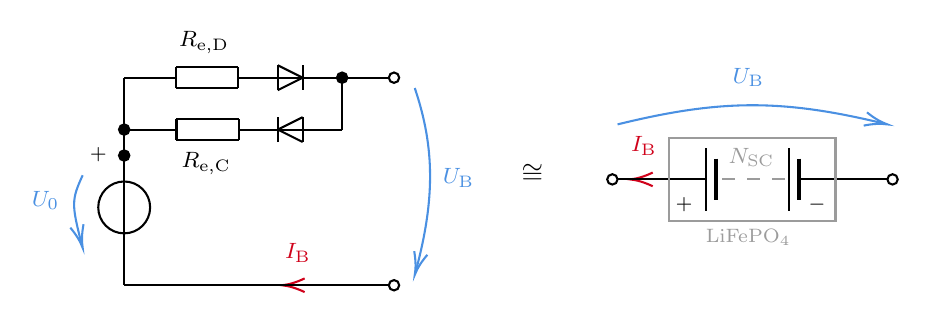
\begin{tikzpicture}[x=0.75pt,y=0.75pt,yscale=-1,xscale=1]
%uncomment if require: \path (0,538); %set diagram left start at 0, and has height of 538

%Straight Lines [id:da4239899953329598] 
\draw [color={rgb, 255:red, 208; green, 2; blue, 27 }  ,draw opacity=1 ]   (353.7,89) -- (340.7,89) ;
\draw [shift={(338.7,89)}, rotate = 360] [color={rgb, 255:red, 208; green, 2; blue, 27 }  ,draw opacity=1 ][line width=0.75]    (10.93,-3.29) .. controls (6.95,-1.4) and (3.31,-0.3) .. (0,0) .. controls (3.31,0.3) and (6.95,1.4) .. (10.93,3.29)   ;
%Straight Lines [id:da9141076711022191] 
\draw    (437.2,89) -- (462.7,89) ;
%Straight Lines [id:da7287140172069071] 
\draw    (332.7,89) -- (358.2,89) ;
%Straight Lines [id:da4302627140031041] 
\draw [line width=0.75]    (375.2,74) -- (375.2,104) ;
%Straight Lines [id:da913986115400165] 
\draw [color={rgb, 255:red, 155; green, 155; blue, 155 }  ,draw opacity=1 ] [dash pattern={on 4.5pt off 4.5pt}]  (413.2,89) -- (378.2,89) ;
%Straight Lines [id:da0409458343135809] 
\draw [line width=1.5]    (380.2,79) -- (380.2,99) ;
%Straight Lines [id:da4345075547353312] 
\draw [line width=0.75]    (415.2,74) -- (415.2,104) ;
%Straight Lines [id:da5169457053238025] 
\draw [line width=1.5]    (420.2,79) -- (420.2,99) ;
%Straight Lines [id:da41248947519842916] 
\draw    (375.2,89) -- (358.2,89) ;
%Straight Lines [id:da6713245296000157] 
\draw    (437.2,89) -- (420.2,89) ;
%Shape: Rectangle [id:dp8204842146016547] 
\draw  [color={rgb, 255:red, 155; green, 155; blue, 155 }  ,draw opacity=1 ] (437.7,69) -- (437.7,109) -- (357.7,109) -- (357.7,69) -- cycle ;
%Shape: Circle [id:dp05668955637455353] 
\draw   (462.7,89) .. controls (462.7,87.62) and (463.82,86.5) .. (465.2,86.5) .. controls (466.58,86.5) and (467.7,87.62) .. (467.7,89) .. controls (467.7,90.38) and (466.58,91.5) .. (465.2,91.5) .. controls (463.82,91.5) and (462.7,90.38) .. (462.7,89) -- cycle ;
%Shape: Circle [id:dp33107549337961006] 
\draw   (327.7,89) .. controls (327.7,87.62) and (328.82,86.5) .. (330.2,86.5) .. controls (331.58,86.5) and (332.7,87.62) .. (332.7,89) .. controls (332.7,90.38) and (331.58,91.5) .. (330.2,91.5) .. controls (328.82,91.5) and (327.7,90.38) .. (327.7,89) -- cycle ;
%Straight Lines [id:da2443541757815666] 
\draw    (150.2,70) -- (150.2,60) ;
%Straight Lines [id:da3018326941100804] 
\draw    (120.2,70) -- (120.2,60) ;
%Straight Lines [id:da09587352502061908] 
\draw    (120.2,60) -- (150.2,60) ;
%Straight Lines [id:da3763833295474801] 
\draw    (120.2,70) -- (150.2,70) ;
%Shape: Circle [id:dp1439179539445421] 
\draw   (222.5,140) .. controls (222.5,138.62) and (223.62,137.5) .. (225,137.5) .. controls (226.38,137.5) and (227.5,138.62) .. (227.5,140) .. controls (227.5,141.38) and (226.38,142.5) .. (225,142.5) .. controls (223.62,142.5) and (222.5,141.38) .. (222.5,140) -- cycle ;
%Curve Lines [id:da3331566122014491] 
\draw [color={rgb, 255:red, 74; green, 144; blue, 226 }  ,draw opacity=1 ]   (235,45) .. controls (244.85,74.06) and (244.67,99.07) .. (235.43,133.42) ;
\draw [shift={(235,135)}, rotate = 285.37] [color={rgb, 255:red, 74; green, 144; blue, 226 }  ,draw opacity=1 ][line width=0.75]    (10.93,-3.29) .. controls (6.95,-1.4) and (3.31,-0.3) .. (0,0) .. controls (3.31,0.3) and (6.95,1.4) .. (10.93,3.29)   ;
%Straight Lines [id:da12346349600905393] 
\draw    (120,65) -- (95,65) ;
%Straight Lines [id:da5810641195940982] 
\draw    (200,65) -- (150,65) ;
%Curve Lines [id:da7444420801068847] 
\draw [color={rgb, 255:red, 74; green, 144; blue, 226 }  ,draw opacity=1 ]   (332.7,62.5) .. controls (382.2,50.32) and (412.1,50.2) .. (461.21,62.13) ;
\draw [shift={(462.7,62.5)}, rotate = 193.82] [color={rgb, 255:red, 74; green, 144; blue, 226 }  ,draw opacity=1 ][line width=0.75]    (10.93,-3.29) .. controls (6.95,-1.4) and (3.31,-0.3) .. (0,0) .. controls (3.31,0.3) and (6.95,1.4) .. (10.93,3.29)   ;
%Straight Lines [id:da5618088487512516] 
\draw    (169,65) -- (169,59) ;
%Straight Lines [id:da29118090532809715] 
\draw    (169,71) -- (169,65) ;
%Straight Lines [id:da2431889749598486] 
\draw    (181,65) -- (181,59) ;
%Straight Lines [id:da9775548645016445] 
\draw    (181,71) -- (181,65) ;
%Straight Lines [id:da3216931327964543] 
\draw    (181,59) -- (169,65) ;
%Straight Lines [id:da870976741839419] 
\draw    (169,65) -- (181,71) ;

%Straight Lines [id:da29875361444983284] 
\draw    (181,40) -- (181,46) ;
%Straight Lines [id:da7309428237562423] 
\draw    (181,34) -- (181,40) ;
%Straight Lines [id:da11204992783900991] 
\draw    (169,40) -- (169,46) ;
%Straight Lines [id:da5502664053025084] 
\draw    (169,34) -- (169,40) ;
%Straight Lines [id:da8629778980345648] 
\draw    (169,46) -- (181,40) ;
%Straight Lines [id:da5424096411610386] 
\draw    (181,40) -- (169,34) ;

%Straight Lines [id:da9431912791064043] 
\draw    (150,45) -- (150,35) ;
%Straight Lines [id:da27346319108632255] 
\draw    (120,45) -- (120,35) ;
%Straight Lines [id:da20640200546003817] 
\draw    (120,35) -- (150,35) ;
%Straight Lines [id:da18589465192348942] 
\draw    (120,45) -- (150,45) ;
%Straight Lines [id:da6749045511361336] 
\draw    (120,40) -- (95,40) ;
%Straight Lines [id:da6054813975075914] 
\draw    (200,40) -- (150,40) ;
%Curve Lines [id:da20601837869887363] 
\draw [color={rgb, 255:red, 74; green, 144; blue, 226 }  ,draw opacity=1 ]   (75,87) .. controls (69.66,98.64) and (69.5,100.87) .. (74.52,120.16) ;
\draw [shift={(75,122)}, rotate = 255.32] [color={rgb, 255:red, 74; green, 144; blue, 226 }  ,draw opacity=1 ][line width=0.75]    (10.93,-3.29) .. controls (6.95,-1.4) and (3.31,-0.3) .. (0,0) .. controls (3.31,0.3) and (6.95,1.4) .. (10.93,3.29)   ;
%Straight Lines [id:da9173542167140516] 
\draw    (95,115) -- (95,140) ;
%Shape: Circle [id:dp7890429606576399] 
\draw   (82.5,102.5) .. controls (82.5,95.6) and (88.1,90) .. (95,90) .. controls (101.9,90) and (107.5,95.6) .. (107.5,102.5) .. controls (107.5,109.4) and (101.9,115) .. (95,115) .. controls (88.1,115) and (82.5,109.4) .. (82.5,102.5) -- cycle ;
%Straight Lines [id:da13008642308028828] 
\draw    (95,90) -- (95,115) ;
%Shape: Circle [id:dp15390548847390928] 
\draw  [fill={rgb, 255:red, 0; green, 0; blue, 0 }  ,fill opacity=1 ] (92.5,65) .. controls (92.5,63.62) and (93.62,62.5) .. (95,62.5) .. controls (96.38,62.5) and (97.5,63.62) .. (97.5,65) .. controls (97.5,66.38) and (96.38,67.5) .. (95,67.5) .. controls (93.62,67.5) and (92.5,66.38) .. (92.5,65) -- cycle ;
%Straight Lines [id:da8926418883187299] 
\draw    (95,65) -- (95,90) ;
%Shape: Circle [id:dp8701642887336025] 
\draw  [fill={rgb, 255:red, 0; green, 0; blue, 0 }  ,fill opacity=1 ] (92.5,77.5) .. controls (92.5,76.12) and (93.62,75) .. (95,75) .. controls (96.38,75) and (97.5,76.12) .. (97.5,77.5) .. controls (97.5,78.88) and (96.38,80) .. (95,80) .. controls (93.62,80) and (92.5,78.88) .. (92.5,77.5) -- cycle ;
%Straight Lines [id:da3048740601702784] 
\draw    (95,40) -- (95,65) ;
%Straight Lines [id:da09511807464774336] 
\draw    (200,40) -- (200,65) ;
%Shape: Circle [id:dp38532315841057274] 
\draw  [fill={rgb, 255:red, 0; green, 0; blue, 0 }  ,fill opacity=1 ] (197.5,40) .. controls (197.5,38.62) and (198.62,37.5) .. (200,37.5) .. controls (201.38,37.5) and (202.5,38.62) .. (202.5,40) .. controls (202.5,41.38) and (201.38,42.5) .. (200,42.5) .. controls (198.62,42.5) and (197.5,41.38) .. (197.5,40) -- cycle ;
%Straight Lines [id:da8764452950084511] 
\draw    (222.5,40) -- (200,40) ;
%Shape: Circle [id:dp3596370907961366] 
\draw   (222.5,40) .. controls (222.5,38.62) and (223.62,37.5) .. (225,37.5) .. controls (226.38,37.5) and (227.5,38.62) .. (227.5,40) .. controls (227.5,41.38) and (226.38,42.5) .. (225,42.5) .. controls (223.62,42.5) and (222.5,41.38) .. (222.5,40) -- cycle ;
%Straight Lines [id:da08595414648708033] 
\draw [color={rgb, 255:red, 208; green, 2; blue, 27 }  ,draw opacity=1 ]   (186,140) -- (173,140) ;
\draw [shift={(171,140)}, rotate = 360] [color={rgb, 255:red, 208; green, 2; blue, 27 }  ,draw opacity=1 ][line width=0.75]    (10.93,-3.29) .. controls (6.95,-1.4) and (3.31,-0.3) .. (0,0) .. controls (3.31,0.3) and (6.95,1.4) .. (10.93,3.29)   ;
%Straight Lines [id:da5785984434842868] 
\draw    (95,140) -- (222.5,140) ;

% Text Node
\draw (373.7,111.4) node [anchor=north west][inner sep=0.75pt]  [font=\scriptsize,color={rgb, 255:red, 0; green, 0; blue, 0 }  ,opacity=1 ]  {$\mathrm{\textcolor[rgb]{0.61,0.61,0.61}{LiFePO}\textcolor[rgb]{0.61,0.61,0.61}{_{4}}}$};
% Text Node
\draw (423.2,96.4) node [anchor=north west][inner sep=0.75pt]  [font=\scriptsize]  {$-$};
% Text Node
\draw (359.2,96.4) node [anchor=north west][inner sep=0.75pt]  [font=\scriptsize]  {$+$};
% Text Node
\draw (384.7,72.4) node [anchor=north west][inner sep=0.75pt]  [font=\footnotesize,color={rgb, 255:red, 155; green, 155; blue, 155 }  ,opacity=1 ]  {$N_{\mathrm{SC}}$};
% Text Node
\draw (285,80.4) node [anchor=north west][inner sep=0.75pt]  [font=\normalsize]  {$\cong $};
% Text Node
\draw (247,82.4) node [anchor=north west][inner sep=0.75pt]  [font=\footnotesize,color={rgb, 255:red, 74; green, 144; blue, 226 }  ,opacity=1 ]  {$U_{\mathrm{B}}$};
% Text Node
\draw (386.7,33.9) node [anchor=north west][inner sep=0.75pt]  [font=\footnotesize,color={rgb, 255:red, 74; green, 144; blue, 226 }  ,opacity=1 ]  {$U_{\mathrm{B}}$};
% Text Node
\draw (337.7,66.9) node [anchor=north west][inner sep=0.75pt]  [font=\footnotesize,color={rgb, 255:red, 208; green, 2; blue, 27 }  ,opacity=1 ]  {$I_{\mathrm{B}}$};
% Text Node
\draw (49,93.4) node [anchor=north west][inner sep=0.75pt]  [font=\footnotesize,color={rgb, 255:red, 74; green, 144; blue, 226 }  ,opacity=1 ]  {$U_{0}$};
% Text Node
\draw (77,71.9) node [anchor=north west][inner sep=0.75pt]  [font=\scriptsize]  {$+$};
% Text Node
\draw (171,118.4) node [anchor=north west][inner sep=0.75pt]  [font=\footnotesize,color={rgb, 255:red, 208; green, 2; blue, 27 }  ,opacity=1 ]  {$I_{\mathrm{B}}$};
% Text Node
\draw (120,16.4) node [anchor=north west][inner sep=0.75pt]  [font=\footnotesize]  {$R_{\mathrm{e,D}}$};
% Text Node
\draw (121.2,74.4) node [anchor=north west][inner sep=0.75pt]  [font=\footnotesize]  {$R_{\mathrm{e,C}}$};


\end{tikzpicture}

	\caption{$R_{\mathrm{int}}$ model of a $\mathrm{LiFePO}_4$ battery (electrochemical energy storage device). (Recreated from: \cite{Hinz:2019, Saldana:2019})}
	\label{fig:tikz_simple_battery_model}
\end{figure}

Figure \ref{fig:tikz_u_oc_vs_soc} shows the typical behavior of the open-circuit voltage $U_0$ of a $\mathrm{LiFePO}_4$ battery as a function of the $\mathrm{SOC}$. For the electrolyte resistances $R_{\mathrm{e,D}}(\mathrm{SOC})$ and $R_{\mathrm{e,C}}(\mathrm{SOC})$, however, it is more difficult to create a generalized function curve. This is due to their varying behavior for different $\mathrm{LiFePO}_4$ batteries \cite{Mertens:2015, Sterner:2017, Li:2018, Hinz:2019, Hossain:2019}. 
\begin{figure}[h!]
	\centering
	

\tikzset{every picture/.style={line width=0.75pt}} %set default line width to 0.75pt        

\begin{tikzpicture}[x=0.75pt,y=0.75pt,yscale=-1,xscale=1]
%uncomment if require: \path (0,300); %set diagram left start at 0, and has height of 300

%Image [id:dp25156695856969735] 
\draw (311.78,133.5) node  {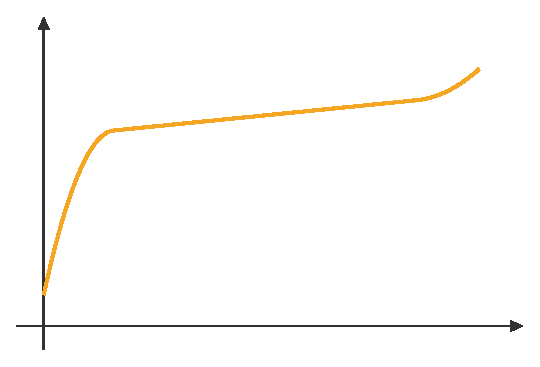
\includegraphics[width=243pt,height=159.75pt]{images/image_u_oc_vs_soc}};
%Straight Lines [id:da24738599691787533] 
\draw [color={rgb, 255:red, 155; green, 155; blue, 155 }  ,draw opacity=1 ] [dash pattern={on 4.5pt off 4.5pt}]  (446.5,59.6) -- (446.23,226.14) ;
%Straight Lines [id:da006125162687165009] 
\draw    (217.33,65) -- (403.33,65) ;
\draw [shift={(405.33,65)}, rotate = 180] [color={rgb, 255:red, 0; green, 0; blue, 0 }  ][line width=0.75]    (10.93,-3.29) .. controls (6.95,-1.4) and (3.31,-0.3) .. (0,0) .. controls (3.31,0.3) and (6.95,1.4) .. (10.93,3.29)   ;
\draw [shift={(215.33,65)}, rotate = 0] [color={rgb, 255:red, 0; green, 0; blue, 0 }  ][line width=0.75]    (10.93,-3.29) .. controls (6.95,-1.4) and (3.31,-0.3) .. (0,0) .. controls (3.31,0.3) and (6.95,1.4) .. (10.93,3.29)   ;
%Straight Lines [id:da953558041904232] 
\draw    (215.33,60) -- (215.33,70) ;
%Straight Lines [id:da48944491555667446] 
\draw    (405.33,60) -- (405.33,70) ;

%Shape: Circle [id:dp3335837862454767] 
\draw  [fill={rgb, 255:red, 255; green, 255; blue, 255 }  ,fill opacity=1 ] (444.5,59.6) .. controls (444.5,58.5) and (445.4,57.6) .. (446.5,57.6) .. controls (447.6,57.6) and (448.5,58.5) .. (448.5,59.6) .. controls (448.5,60.7) and (447.6,61.6) .. (446.5,61.6) .. controls (445.4,61.6) and (444.5,60.7) .. (444.5,59.6) -- cycle ;
%Shape: Circle [id:dp5046748837393529] 
\draw  [fill={rgb, 255:red, 255; green, 255; blue, 255 }  ,fill opacity=1 ] (165.3,202.93) .. controls (165.3,201.83) and (166.2,200.93) .. (167.3,200.93) .. controls (168.4,200.93) and (169.3,201.83) .. (169.3,202.93) .. controls (169.3,204.04) and (168.4,204.93) .. (167.3,204.93) .. controls (166.2,204.93) and (165.3,204.04) .. (165.3,202.93) -- cycle ;
%Shape: Circle [id:dp5166078562699203] 
\draw  [fill={rgb, 255:red, 255; green, 255; blue, 255 }  ,fill opacity=1 ] (175.5,162.27) .. controls (175.5,161.16) and (176.4,160.27) .. (177.5,160.27) .. controls (178.6,160.27) and (179.5,161.16) .. (179.5,162.27) .. controls (179.5,163.37) and (178.6,164.27) .. (177.5,164.27) .. controls (176.4,164.27) and (175.5,163.37) .. (175.5,162.27) -- cycle ;

% Text Node
\draw (142.5,5.4) node [anchor=north west][inner sep=0.75pt]  [font=\footnotesize]  {$U_{0}(\mathrm{SOC})$};
% Text Node
\draw (478.5,218.4) node [anchor=north west][inner sep=0.75pt]  [font=\footnotesize]  {$\mathrm{SOC}$};
% Text Node
\draw (153.33,229.07) node [anchor=north west][inner sep=0.75pt]  [font=\footnotesize]  {$0$};
% Text Node
\draw (441.67,228.4) node [anchor=north west][inner sep=0.75pt]  [font=\footnotesize]  {$1$};
% Text Node
\draw (280,47.4) node [anchor=north west][inner sep=0.75pt]  [font=\footnotesize]  {$\approx \text{Linear}$};
% Text Node
\draw (454,53.4) node [anchor=north west][inner sep=0.75pt]  [font=\footnotesize]  {$\mathrm{SOC}_{N_{\mathrm{MP}}}$};
% Text Node
\draw (186,157.4) node [anchor=north west][inner sep=0.75pt]  [font=\footnotesize]  {$\mathrm{SOC}_{2}$};
% Text Node
\draw (176,197.4) node [anchor=north west][inner sep=0.75pt]  [font=\footnotesize]  {$\mathrm{SOC}_{1}$};
% Text Node
\draw (202.6,138.98) node [anchor=north west][inner sep=0.75pt]  [font=\footnotesize,rotate=-292]  {$\dotsc $};


\end{tikzpicture}



	\caption{Typical behavior of the open-circuit voltage $U_0$ of a $\mathrm{LiFePO}_4$ battery depending on the $\mathrm{SOC}$. $\mathrm{SOC_1}$ to $\mathrm{SOC}_{N_\mathrm{MP}}$ represent the measuring points for the discharging and charging experiment. (Recreated from: \cite{Mertens:2015, Sterner:2017, Li:2018, Hinz:2019, Hossain:2019})}
	\label{fig:tikz_u_oc_vs_soc}
\end{figure}

On this basis, the terminal voltage of the battery $U_\mathrm{B}$ as a function of the SOC, and wether it is being discharged or charged, can be obtained after Kirchhoff's second law is applied to the model \cite{He:2011, Wehbe:2015, Hinz:2019, Saldana:2019}:
	\begin{equation} \label{eq:battery_voltage}
	\centering
		U_\mathrm{B}(\mathrm{SOC}) =
  		\begin{cases}
   			U_0 - R_{\mathrm{e,D}} \, I_\mathrm{D}\text{,} & \text{when discharging the battery} \\
    		U_0 + R_{\mathrm{e,C}} \, I_\mathrm{C}\text{,} & \text{when charging the battery.}
  		\end{cases}
	\end{equation} 
	
At this point it must be made clear that a $\mathrm{LiFePO}_4$ battery is completely discharged when the voltage $U_\mathrm{B} = U_\mathrm{cut-off}$ is reached and fully charged when the voltage $U_\mathrm{B} = U_\mathrm{full}$ is reached \cite{Hinz:2019, Offgridtec:2020}.\footnote{The name \emph{cuf-off voltage} comes from the fact that the BMS turns off the battery to avoid an unsafe state.} If the equations (\ref{eq:battery_voltage}) and (\ref{eq:battery_charge}) are compared, it can be seen that $U_\mathrm{cut-off}$ is reached at a later point in time for smaller currents $I_\mathrm{D}$. This shows that the battery can be discharged more deeply, which manifests itself in a larger total available battery charge $Q_\mathrm{B}$ \cite{Hausmann:2013, Kurzweil:2018}. Here, however, the compromise is made that the cut-off voltage in the proposed model varies for different discharging currents. 

Figure \ref{fig:tikz_pc_pd_battery_curve} shows the behavior of the battery voltage $U_{\mathrm B}(t)$ when it is discharged with a constant current $I_{\mathrm D}$ over the \emph{time interval} $\Delta t_{\mathrm{D}} = t_\mathrm{D, off} - t_\mathrm{D, on}$ in $\left(\mathrm{h}\right)$ and then charged with the constant current $I_{\mathrm C}$ over the time interval $\Delta t_{\mathrm{C}} = t_\mathrm{C, off} - t_\mathrm{C, on}$ in $\left(\mathrm{h}\right)$ \cite{Rahmoun:2012, Hentunen:2014, Li:2018, Kurzweil:2018, Gurjer:2019, Saldana:2019, Hossain:2019}.
\begin{figure}[h!]
	\centering
	

\tikzset{every picture/.style={line width=0.75pt}} %set default line width to 0.75pt        

\begin{tikzpicture}[x=0.75pt,y=0.75pt,yscale=-1,xscale=1]
%uncomment if require: \path (0,399); %set diagram left start at 0, and has height of 399

%Image [id:dp9431825859465086] 
\draw (257.75,202.7) node  {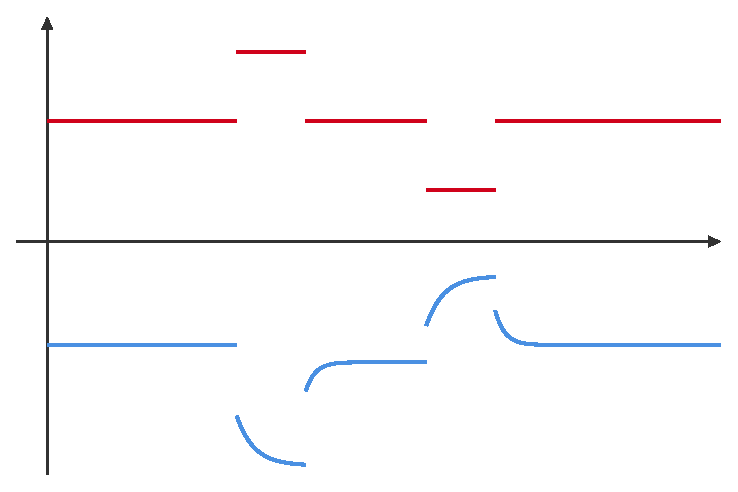
\includegraphics[width=337.88pt,height=219.75pt]{images/image_pc_pd_curve}};
%Straight Lines [id:da7984917488209211] 
\draw [color={rgb, 255:red, 155; green, 155; blue, 155 }  ,draw opacity=1 ] [dash pattern={on 4.5pt off 4.5pt}]  (285,265.7) -- (435,265.7) ;
%Straight Lines [id:da23770186298412455] 
\draw [color={rgb, 255:red, 155; green, 155; blue, 155 }  ,draw opacity=1 ] [dash pattern={on 4.5pt off 4.5pt}]  (59,265.7) -- (250,265.7) ;
%Straight Lines [id:da8950127464122881] 
\draw [color={rgb, 255:red, 74; green, 144; blue, 226 }  ,draw opacity=1 ][line width=1.5]  [dash pattern={on 1.69pt off 2.76pt}]  (173,269.5) -- (173,307.5) ;
%Straight Lines [id:da8271633433271262] 
\draw [color={rgb, 255:red, 74; green, 144; blue, 226 }  ,draw opacity=1 ][line width=1.5]  [dash pattern={on 1.69pt off 2.76pt}]  (217,299.2) -- (217,337.2) ;
%Straight Lines [id:da6802360531812348] 
\draw [color={rgb, 255:red, 74; green, 144; blue, 226 }  ,draw opacity=1 ][line width=1.5]  [dash pattern={on 1.69pt off 2.76pt}]  (294,257) -- (294,272) ;
%Straight Lines [id:da665320735281528] 
\draw [color={rgb, 255:red, 74; green, 144; blue, 226 }  ,draw opacity=1 ][line width=1.5]  [dash pattern={on 1.69pt off 2.76pt}]  (338.5,226) -- (338.5,241) ;
%Straight Lines [id:da5155481731261737] 
\draw [color={rgb, 255:red, 208; green, 2; blue, 27 }  ,draw opacity=1 ][line width=1.5]  [dash pattern={on 1.69pt off 2.76pt}]  (173.5,84.5) -- (173.5,119.5) ;
%Straight Lines [id:da010424395564271549] 
\draw [color={rgb, 255:red, 208; green, 2; blue, 27 }  ,draw opacity=1 ][line width=1.5]  [dash pattern={on 1.69pt off 2.76pt}]  (217.5,85.5) -- (217.5,120.5) ;
%Straight Lines [id:da3234870226616544] 
\draw [color={rgb, 255:red, 208; green, 2; blue, 27 }  ,draw opacity=1 ][line width=1.5]  [dash pattern={on 1.69pt off 2.76pt}]  (295,128.5) -- (295,163.5) ;
%Straight Lines [id:da1669627999747061] 
\draw [color={rgb, 255:red, 208; green, 2; blue, 27 }  ,draw opacity=1 ][line width=1.5]  [dash pattern={on 1.69pt off 2.76pt}]  (338.5,128.5) -- (338.5,163.5) ;
%Straight Lines [id:da7336073832767973] 
\draw [color={rgb, 255:red, 155; green, 155; blue, 155 }  ,draw opacity=1 ] [dash pattern={on 4.5pt off 4.5pt}]  (180.5,122.5) -- (216.5,122.5) ;
%Straight Lines [id:da38951316698254357] 
\draw    (231,339.63) -- (231,299.5) ;
\draw [shift={(231,297.5)}, rotate = 450] [color={rgb, 255:red, 0; green, 0; blue, 0 }  ][line width=0.75]    (10.93,-3.29) .. controls (6.95,-1.4) and (3.31,-0.3) .. (0,0) .. controls (3.31,0.3) and (6.95,1.4) .. (10.93,3.29)   ;
\draw [shift={(231,341.63)}, rotate = 270] [color={rgb, 255:red, 0; green, 0; blue, 0 }  ][line width=0.75]    (10.93,-3.29) .. controls (6.95,-1.4) and (3.31,-0.3) .. (0,0) .. controls (3.31,0.3) and (6.95,1.4) .. (10.93,3.29)   ;
%Straight Lines [id:da35829040806212764] 
\draw    (236,342.16) -- (226,342.16) ;

%Straight Lines [id:da8393771568930704] 
\draw    (226,297) -- (236,297) ;

%Straight Lines [id:da20675405566740057] 
\draw [color={rgb, 255:red, 155; green, 155; blue, 155 }  ,draw opacity=1 ] [dash pattern={on 4.5pt off 4.5pt}]  (58,78.5) -- (169,78.5) ;
%Straight Lines [id:da3893499978016637] 
\draw [color={rgb, 255:red, 155; green, 155; blue, 155 }  ,draw opacity=1 ] [dash pattern={on 4.5pt off 4.5pt}]  (57,166.7) -- (291,166.7) ;
%Straight Lines [id:da14032166669051893] 
\draw [color={rgb, 255:red, 54; green, 162; blue, 138 }  ,draw opacity=1 ]   (52.2,265.7) -- (173,265.7) ;
%Straight Lines [id:da830483625109742] 
\draw [color={rgb, 255:red, 54; green, 162; blue, 138 }  ,draw opacity=1 ]   (173,265.7) -- (173,310.7) ;
%Straight Lines [id:da8193661154783456] 
\draw [color={rgb, 255:red, 54; green, 162; blue, 138 }  ,draw opacity=1 ]   (217,276.7) -- (294,276.7) ;
%Straight Lines [id:da5334736769051522] 
\draw [color={rgb, 255:red, 54; green, 162; blue, 138 }  ,draw opacity=1 ]   (217,276.7) -- (217,321.7) ;
%Straight Lines [id:da910430036604543] 
\draw [color={rgb, 255:red, 54; green, 162; blue, 138 }  ,draw opacity=1 ]   (173,310.7) -- (217,321.7) ;
%Straight Lines [id:da21771101198750498] 
\draw [color={rgb, 255:red, 54; green, 162; blue, 138 }  ,draw opacity=1 ]   (294,253.7) -- (294,276.7) ;
%Straight Lines [id:da8239917812667736] 
\draw [color={rgb, 255:red, 54; green, 162; blue, 138 }  ,draw opacity=1 ]   (311,330) -- (336,330) ;
%Straight Lines [id:da009949911281480484] 
\draw [color={rgb, 255:red, 54; green, 162; blue, 138 }  ,draw opacity=1 ]   (338.5,242.7) -- (338.5,265.7) ;
%Straight Lines [id:da553277774653504] 
\draw [color={rgb, 255:red, 54; green, 162; blue, 138 }  ,draw opacity=1 ]   (338.5,265.7) -- (482.7,265.7) ;
%Straight Lines [id:da4348739238851991] 
\draw [color={rgb, 255:red, 54; green, 162; blue, 138 }  ,draw opacity=1 ]   (294,253.7) -- (338.5,242.7) ;
%Straight Lines [id:da536977341179073] 
\draw [color={rgb, 255:red, 155; green, 155; blue, 155 }  ,draw opacity=1 ] [dash pattern={on 4.5pt off 4.5pt}]  (301,122.5) -- (337,122.5) ;
%Straight Lines [id:da4017649297581949] 
\draw    (280.89,237.56) -- (280.89,252.56) ;
%Straight Lines [id:da6514598025702074] 
\draw    (351.45,204.9) -- (351.45,219.9) ;
%Straight Lines [id:da6789214017371121] 
\draw    (351.45,245.68) -- (351.45,260.68) ;
%Straight Lines [id:da8572632508349955] 
\draw    (280.89,276.33) -- (280.89,254.56) ;
\draw [shift={(280.89,254.56)}, rotate = 270] [color={rgb, 255:red, 0; green, 0; blue, 0 }  ][line width=0.75]    (10.93,-3.29) .. controls (6.95,-1.4) and (3.31,-0.3) .. (0,0) .. controls (3.31,0.3) and (6.95,1.4) .. (10.93,3.29)   ;
\draw [shift={(280.89,276.33)}, rotate = 450] [color={rgb, 255:red, 0; green, 0; blue, 0 }  ][line width=0.75]    (10.93,-3.29) .. controls (6.95,-1.4) and (3.31,-0.3) .. (0,0) .. controls (3.31,0.3) and (6.95,1.4) .. (10.93,3.29)   ;
%Straight Lines [id:da6742965413146893] 
\draw    (285.89,254.27) -- (275.89,254.27) ;
%Straight Lines [id:da3735265920193138] 
\draw    (275.89,276.61) -- (285.89,276.61) ;

%Straight Lines [id:da4089848528137756] 
\draw    (280.89,278.33) -- (280.89,293.33) ;
%Straight Lines [id:da6377765727461617] 
\draw    (351.45,243.68) -- (351.45,221.9) ;
\draw [shift={(351.45,221.9)}, rotate = 270] [color={rgb, 255:red, 0; green, 0; blue, 0 }  ][line width=0.75]    (10.93,-3.29) .. controls (6.95,-1.4) and (3.31,-0.3) .. (0,0) .. controls (3.31,0.3) and (6.95,1.4) .. (10.93,3.29)   ;
\draw [shift={(351.45,243.68)}, rotate = 450] [color={rgb, 255:red, 0; green, 0; blue, 0 }  ][line width=0.75]    (10.93,-3.29) .. controls (6.95,-1.4) and (3.31,-0.3) .. (0,0) .. controls (3.31,0.3) and (6.95,1.4) .. (10.93,3.29)   ;
%Straight Lines [id:da4999891213389307] 
\draw    (356.45,221.62) -- (346.45,221.62) ;
%Straight Lines [id:da21342574530244263] 
\draw    (346.45,243.96) -- (356.45,243.96) ;

%Straight Lines [id:da38332448511266115] 
\draw    (160.11,308.3) -- (160.11,268.17) ;
\draw [shift={(160.11,266.17)}, rotate = 450] [color={rgb, 255:red, 0; green, 0; blue, 0 }  ][line width=0.75]    (10.93,-3.29) .. controls (6.95,-1.4) and (3.31,-0.3) .. (0,0) .. controls (3.31,0.3) and (6.95,1.4) .. (10.93,3.29)   ;
\draw [shift={(160.11,310.3)}, rotate = 270] [color={rgb, 255:red, 0; green, 0; blue, 0 }  ][line width=0.75]    (10.93,-3.29) .. controls (6.95,-1.4) and (3.31,-0.3) .. (0,0) .. controls (3.31,0.3) and (6.95,1.4) .. (10.93,3.29)   ;
%Straight Lines [id:da5321486664645252] 
\draw    (165.11,310.83) -- (155.11,310.83) ;

%Straight Lines [id:da08166456175406989] 
\draw    (155.11,265.67) -- (165.11,265.67) ;

%Straight Lines [id:da5101730964523248] 
\draw    (173,195.5) -- (173,203.5) ;
%Straight Lines [id:da2319819541264927] 
\draw    (217,195.5) -- (217,203.5) ;
%Straight Lines [id:da808601911633186] 
\draw    (295,195.5) -- (295,203.5) ;
%Straight Lines [id:da3828209146801427] 
\draw    (339,195.5) -- (339,203.5) ;
%Straight Lines [id:da8203400723269536] 
\draw [color={rgb, 255:red, 208; green, 2; blue, 27 }  ,draw opacity=1 ]   (17,21.33) -- (42,21.33) ;
%Straight Lines [id:da38547811974611657] 
\draw [color={rgb, 255:red, 74; green, 144; blue, 226 }  ,draw opacity=1 ]   (17,41.33) -- (42,41.33) ;


% Text Node
\draw (488,193.4) node [anchor=north west][inner sep=0.75pt]  [font=\footnotesize]  {$t$};
% Text Node
\draw (32,160.4) node [anchor=north west][inner sep=0.75pt]  [font=\footnotesize]  {$I_{\mathrm{C}}$};
% Text Node
\draw (32,73.4) node [anchor=north west][inner sep=0.75pt]  [font=\footnotesize]  {$I_{\mathrm{D}}$};
% Text Node
\draw (29,120.4) node [anchor=north west][inner sep=0.75pt]  [font=\footnotesize]  {$0\mathrm{A}$};
% Text Node
\draw (56.7,245.4) node [anchor=north west][inner sep=0.75pt]  [font=\footnotesize]  {$U_{0}( t=0\mathrm{s})$};
% Text Node
\draw (32.82,205.54) node [anchor=north west][inner sep=0.75pt]  [font=\footnotesize]  {$0\mathrm{s}$};
% Text Node
\draw (125.89,280.96) node [anchor=north west][inner sep=0.75pt]  [font=\footnotesize]  {$\Delta U_{\mathrm{D}}$};
% Text Node
\draw (235.22,313.18) node [anchor=north west][inner sep=0.75pt]  [font=\footnotesize]  {$\Delta U_{\mathrm{D}}$};
% Text Node
\draw (355.3,226.79) node [anchor=north west][inner sep=0.75pt]  [font=\footnotesize]  {$\Delta U_{\mathrm{C}}$};
% Text Node
\draw (248.11,259.57) node [anchor=north west][inner sep=0.75pt]  [font=\footnotesize]  {$\Delta U_{\mathrm{C}}$};
% Text Node
\draw (340,323.4) node [anchor=north west][inner sep=0.75pt]  [font=\footnotesize]  {$U_{\mathrm{B}}( t)\text{ with the } R_{\mathrm{int}}\text{ model}$};
% Text Node
\draw (159,56) node [anchor=north west][inner sep=0.75pt]  [font=\footnotesize] [align=left] {Discharging};
% Text Node
\draw (287.33,100.5) node [anchor=north west][inner sep=0.75pt]  [font=\footnotesize] [align=left] {Charging};
% Text Node
\draw (162.8,178.8) node [anchor=north west][inner sep=0.75pt]  [font=\footnotesize]  {$t_{\mathrm{D} ,\mathrm{on}}$};
% Text Node
\draw (206.4,178.8) node [anchor=north west][inner sep=0.75pt]  [font=\footnotesize]  {$t_{\mathrm{D} ,\mathrm{off}}$};
% Text Node
\draw (285,178.8) node [anchor=north west][inner sep=0.75pt]  [font=\footnotesize]  {$t_{\mathrm{C} ,\mathrm{on}}$};
% Text Node
\draw (328.8,178.8) node [anchor=north west][inner sep=0.75pt]  [font=\footnotesize]  {$t_{\mathrm{C} ,\mathrm{off}}$};
% Text Node
\draw (45,14.73) node [anchor=north west][inner sep=0.75pt]  [font=\footnotesize]  {$I_{\mathrm{B}}( t)$};
% Text Node
\draw (45,34.73) node [anchor=north west][inner sep=0.75pt]  [font=\footnotesize]  {$U_{\mathrm{B}}( t)$};


\end{tikzpicture}




	\caption{Behavior of the battery voltage $U_{\mathrm B}(t)$ when it is first discharged with $I_{\mathrm D}$ and then charged with $I_{\mathrm C}$. From the resulting voltage drop $\Delta U_{\mathrm D}(t_\mathrm{D, on})$ and voltage rise $\Delta U_{\mathrm C}(t_\mathrm{C, on})$, the $R_{int}$ model's electrolyte resistances $R_{e,\mathrm{D}}$ and $R_{e,\mathrm{C}}$ can be calculated. The turquoise curve represents the behavior of the modeled battery voltage. (Recreated from: \cite{Rahmoun:2012, Hentunen:2014, Li:2018, Kurzweil:2018, Gurjer:2019, Saldana:2019, Hossain:2019})}
	\label{fig:tikz_pc_pd_battery_curve}
\end{figure}
From the \emph{dropping voltages} $\Delta U_{\mathrm D}(t_\mathrm{D, on})$ and $\Delta U_{\mathrm C}(t_\mathrm{C, off})$ or \emph{rising voltages} $\Delta U_{\mathrm D}(t_\mathrm{D, off})$ and $\Delta U_{\mathrm C}(t_\mathrm{C, on})$ in $\left( \mathrm{V} \right)$, the $R_{int}$ model's electrolyte resistances $R_{\mathrm{e,D}}$ and $R_{\mathrm{e,C}}$ can be calculated as shown in the equations (\ref{eq:r_0_d}) and (\ref{eq:r_0_c}) \cite{Rahmoun:2012, Hentunen:2014, Kurzweil:2018, Gurjer:2019}. 
\begin{equation}\label{eq:r_0_d}
	\centering
	R_{\mathrm{e,D}}(t) = \left|\dfrac{\Delta U_{\mathrm D}}{I_{\mathrm D}}\right|
\end{equation}
\begin{equation}\label{eq:r_0_c}
	\centering
	R_{\mathrm{e,C}}(t) = \left|\dfrac{\Delta U_{\mathrm C}}{I_{\mathrm C}}\right|
\end{equation}
For comparison, the thin turquoise curve represents the behavior of the $R_\mathrm{int}$ model for the same discharge and charge currents $I_{\mathrm D}$ and $I_{\mathrm C}$. At times $t_\mathrm{D, on}$, $t_\mathrm{D, off}$, $t_\mathrm{C, on}$ and $t_\mathrm{C, off}$ it has the same dropping and rising voltages $\Delta U_{\mathrm D}$ and $\Delta U_{\mathrm C}$ as $U_{\mathrm B}(t)$ \cite{Saldana:2019}.

Based on the findings in the articles \cite{Hausmann:2013, Ala-A.-Hussein:2015, Nejad:2016, Chin:2018} it is assumed that $U_0$,  $R_{e,\mathrm{D}}$ and $R_{e,\mathrm{C}}$ do not dependent on the ambient temperature $\vartheta_{\mathrm{A}}$ in the range from $5^\circ \mathrm{C}$ to $45^\circ \mathrm{C}$. Therefore, the proposed model does not apply to temperatures below $5^\circ \mathrm{C}$ and above $45^\circ \mathrm{C}$.

In order to complete the $R_{\mathrm{int}}$ model, the missing properties $U_0(\mathrm{SOC})$, $R_{\mathrm{e,D}}(\mathrm{SOC})$ and $R_{\mathrm{e,C}}(\mathrm{SOC})$ must be determined experimentally. For this purpose, two separate experiments must be carried out as explained in the following paragraphs.

\paragraph*{Discharging experiment:} %% PD EXPERIMENT
The experiment is carried out at the ambient temperature $\vartheta_\mathrm{A} = 25^\circ \mathrm{C}$ with an initially fully charged $\mathrm{LiFePO}_4$ battery ($\mathrm{SOC}_{N_\mathrm{MP}} = 1$) and repeated for the desired \emph{number of measuring points} $N_{\mathrm{MP}}$ in $\left( 1 \right)$, as illustrated in the figure \ref{fig:tikz_u_oc_vs_soc}, until the battery is fully discharged ($\mathrm{SOC}_{1} = 0$) \cite{Rahmoun:2012, Hentunen:2014, Gurjer:2019}. 

A simple measurement setup for this experiment can be seen in the figure \ref{fig:tikz_experiment_1}. $U_\mathrm{shunt}$ in $\left(\mathrm{V}\right)$ is the voltage drop across the shunt resistor $R_\mathrm{shunt}$, measured with \emph{channel 2} (Ch2) of the oscilloscope. On the basis of this voltage drop, $I_\mathrm{L}$ is set so that the battery is discharged with the current:
\begin{equation}\label{eq_i_d_real}
	\centering
I_\mathrm{D} = \dfrac{U_\mathrm{shunt}}{R_\mathrm{shunt}} + I_\mathrm{Ch1} + I_\mathrm{Ch2} \text{.}
\end{equation}
The \emph{measuring currents} $I_\mathrm{Ch1}$ and $I_\mathrm{Ch2}$ in $\left(\mathrm{A}\right)$ caused by the internal resistances of the channels of the oscilloscope are small compared to the load current $I_\mathrm{L}$. Depending on the desired accuracy, $I_\mathrm{Ch1}$ and $I_\mathrm{Ch2}$ can either be neglected or determined by measuring the internal resistances of said channels \cite{Schrufer:2014}.  
\begin{figure}[h!]
	\centering
	

\tikzset{every picture/.style={line width=0.75pt}} %set default line width to 0.75pt        

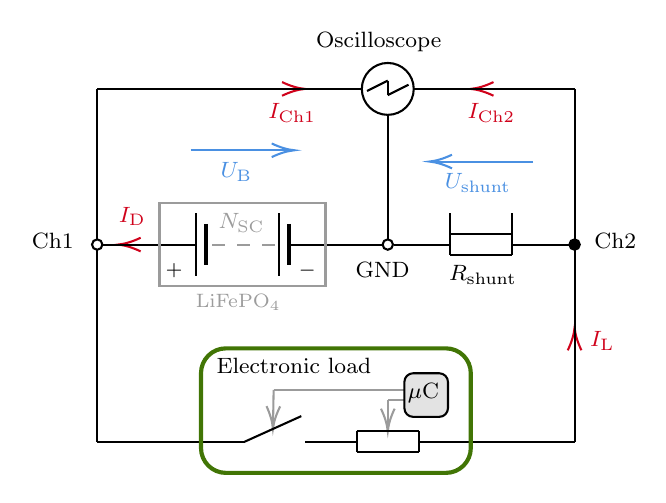
\begin{tikzpicture}[x=0.75pt,y=0.75pt,yscale=-1,xscale=1]
%uncomment if require: \path (0,743); %set diagram left start at 0, and has height of 743

%Straight Lines [id:da045931729156849066] 
\draw [color={rgb, 255:red, 208; green, 2; blue, 27 }  ,draw opacity=1 ]   (285,105) -- (272,105) ;
\draw [shift={(270,105)}, rotate = 360] [color={rgb, 255:red, 208; green, 2; blue, 27 }  ,draw opacity=1 ][line width=0.75]    (10.93,-3.29) .. controls (6.95,-1.4) and (3.31,-0.3) .. (0,0) .. controls (3.31,0.3) and (6.95,1.4) .. (10.93,3.29)   ;
%Straight Lines [id:da3949134308814568] 
\draw    (270,275) -- (320,275) ;
%Straight Lines [id:da08560996153222833] 
\draw [color={rgb, 255:red, 208; green, 2; blue, 27 }  ,draw opacity=1 ]   (115,180) -- (102,180) ;
\draw [shift={(100,180)}, rotate = 360] [color={rgb, 255:red, 208; green, 2; blue, 27 }  ,draw opacity=1 ][line width=0.75]    (10.93,-3.29) .. controls (6.95,-1.4) and (3.31,-0.3) .. (0,0) .. controls (3.31,0.3) and (6.95,1.4) .. (10.93,3.29)   ;
%Straight Lines [id:da050616828595225094] 
\draw    (92.5,180) -- (120.5,180) ;
%Straight Lines [id:da6370801814614784] 
\draw    (200.5,180) -- (227.5,180) ;
%Straight Lines [id:da4527627205165792] 
\draw [color={rgb, 255:red, 208; green, 2; blue, 27 }  ,draw opacity=1 ]   (320,235) -- (320,222) ;
\draw [shift={(320,220)}, rotate = 450] [color={rgb, 255:red, 208; green, 2; blue, 27 }  ,draw opacity=1 ][line width=0.75]    (10.93,-3.29) .. controls (6.95,-1.4) and (3.31,-0.3) .. (0,0) .. controls (3.31,0.3) and (6.95,1.4) .. (10.93,3.29)   ;
%Straight Lines [id:da4189378099752894] 
\draw [color={rgb, 255:red, 208; green, 2; blue, 27 }  ,draw opacity=1 ]   (175,105) -- (188,105) ;
\draw [shift={(190,105)}, rotate = 180] [color={rgb, 255:red, 208; green, 2; blue, 27 }  ,draw opacity=1 ][line width=0.75]    (10.93,-3.29) .. controls (6.95,-1.4) and (3.31,-0.3) .. (0,0) .. controls (3.31,0.3) and (6.95,1.4) .. (10.93,3.29)   ;
%Straight Lines [id:da2658092860751087] 
\draw [line width=0.75]    (137.5,165) -- (137.5,195) ;
%Straight Lines [id:da3949939895399093] 
\draw [color={rgb, 255:red, 155; green, 155; blue, 155 }  ,draw opacity=1 ] [dash pattern={on 4.5pt off 4.5pt}]  (175.5,180) -- (140.5,180) ;
%Straight Lines [id:da6668323928749316] 
\draw [line width=1.5]    (142.5,170) -- (142.5,190) ;
%Straight Lines [id:da2892580654722863] 
\draw [line width=0.75]    (177.5,165) -- (177.5,195) ;
%Straight Lines [id:da305974803365608] 
\draw [line width=1.5]    (182.5,170) -- (182.5,190) ;
%Straight Lines [id:da02397573109880402] 
\draw    (137.5,180) -- (120.5,180) ;
%Straight Lines [id:da31190085768960363] 
\draw    (199.5,180) -- (182.5,180) ;
%Shape: Rectangle [id:dp8008725070360889] 
\draw  [color={rgb, 255:red, 155; green, 155; blue, 155 }  ,draw opacity=1 ] (200,160) -- (200,200) -- (120,200) -- (120,160) -- cycle ;
%Shape: Circle [id:dp20223673484144356] 
\draw   (227.5,180) .. controls (227.5,178.62) and (228.62,177.5) .. (230,177.5) .. controls (231.38,177.5) and (232.5,178.62) .. (232.5,180) .. controls (232.5,181.38) and (231.38,182.5) .. (230,182.5) .. controls (228.62,182.5) and (227.5,181.38) .. (227.5,180) -- cycle ;
%Shape: Circle [id:dp3853206170680481] 
\draw   (87.5,180) .. controls (87.5,178.62) and (88.62,177.5) .. (90,177.5) .. controls (91.38,177.5) and (92.5,178.62) .. (92.5,180) .. controls (92.5,181.38) and (91.38,182.5) .. (90,182.5) .. controls (88.62,182.5) and (87.5,181.38) .. (87.5,180) -- cycle ;
%Straight Lines [id:da5327428480980583] 
\draw    (90,105) -- (90,177.5) ;
%Straight Lines [id:da13935190161788125] 
\draw    (90,105) -- (217.5,105) ;
%Straight Lines [id:da7865577264880768] 
\draw [color={rgb, 255:red, 74; green, 144; blue, 226 }  ,draw opacity=1 ]   (135,134.57) -- (183,134.57) ;
\draw [shift={(185,134.57)}, rotate = 180] [color={rgb, 255:red, 74; green, 144; blue, 226 }  ,draw opacity=1 ][line width=0.75]    (10.93,-3.29) .. controls (6.95,-1.4) and (3.31,-0.3) .. (0,0) .. controls (3.31,0.3) and (6.95,1.4) .. (10.93,3.29)   ;
%Shape: Circle [id:dp3317910125615249] 
\draw   (217.5,105) .. controls (217.5,98.1) and (223.1,92.5) .. (230,92.5) .. controls (236.9,92.5) and (242.5,98.1) .. (242.5,105) .. controls (242.5,111.9) and (236.9,117.5) .. (230,117.5) .. controls (223.1,117.5) and (217.5,111.9) .. (217.5,105) -- cycle ;
%Straight Lines [id:da1875474942123041] 
\draw    (220,106) -- (230,101) ;
%Straight Lines [id:da4090541258718201] 
\draw    (230,101) -- (230,108) ;
%Straight Lines [id:da7457893967384179] 
\draw    (230,108) -- (240,103) ;

%Straight Lines [id:da0917057683123701] 
\draw    (90,182.5) -- (90,275) ;
%Straight Lines [id:da2778004994432466] 
\draw [color={rgb, 255:red, 155; green, 155; blue, 155 }  ,draw opacity=1 ]   (230,255) -- (230,268) ;
\draw [shift={(230,270)}, rotate = 270] [color={rgb, 255:red, 155; green, 155; blue, 155 }  ,draw opacity=1 ][line width=0.75]    (10.93,-3.29) .. controls (6.95,-1.4) and (3.31,-0.3) .. (0,0) .. controls (3.31,0.3) and (6.95,1.4) .. (10.93,3.29)   ;
%Straight Lines [id:da32924484737520543] 
\draw    (245,280) -- (245,270) ;
%Straight Lines [id:da33462944952545204] 
\draw    (215,280) -- (215,270) ;
%Straight Lines [id:da24868968049308626] 
\draw    (215,270) -- (245,270) ;
%Straight Lines [id:da6617574409624216] 
\draw    (215,280) -- (245,280) ;
%Straight Lines [id:da8690193038101492] 
\draw    (215,275) -- (200,275) ;
%Straight Lines [id:da7998432795618544] 
\draw [color={rgb, 255:red, 155; green, 155; blue, 155 }  ,draw opacity=1 ]   (238,255) -- (230,255) ;
%Straight Lines [id:da10758294037064475] 
\draw    (270,275) -- (245,275) ;
%Straight Lines [id:da6790087801319198] 
\draw    (90,275) -- (140,275) ;
%Straight Lines [id:da7635403190384071] 
\draw [color={rgb, 255:red, 155; green, 155; blue, 155 }  ,draw opacity=1 ]   (174.71,266.83) -- (175,250) ;
\draw [shift={(174.67,268.83)}, rotate = 271] [color={rgb, 255:red, 155; green, 155; blue, 155 }  ,draw opacity=1 ][line width=0.75]    (10.93,-3.29) .. controls (6.95,-1.4) and (3.31,-0.3) .. (0,0) .. controls (3.31,0.3) and (6.95,1.4) .. (10.93,3.29)   ;
%Straight Lines [id:da09729743826270276] 
\draw    (205,275) -- (190,275) ;
%Straight Lines [id:da1421569585710698] 
\draw    (188.34,262.65) -- (161,275) ;
%Straight Lines [id:da5452375072503128] 
\draw    (161,275) -- (140,275) ;
%Straight Lines [id:da5345291081584591] 
\draw [color={rgb, 255:red, 155; green, 155; blue, 155 }  ,draw opacity=1 ]   (238,250) -- (175,250) ;
%Rounded Rect [id:dp6576837931168715] 
\draw  [fill={rgb, 255:red, 227; green, 227; blue, 227 }  ,fill opacity=1 ] (238,246.2) .. controls (238,243.88) and (239.88,242) .. (242.2,242) -- (254.8,242) .. controls (257.12,242) and (259,243.88) .. (259,246.2) -- (259,258.8) .. controls (259,261.12) and (257.12,263) .. (254.8,263) -- (242.2,263) .. controls (239.88,263) and (238,261.12) .. (238,258.8) -- cycle ;

%Rounded Rect [id:dp11415612065842651] 
\draw  [color={rgb, 255:red, 65; green, 117; blue, 5 }  ,draw opacity=1 ][line width=1.5]  (140,242) .. controls (140,235.37) and (145.37,230) .. (152,230) -- (258,230) .. controls (264.63,230) and (270,235.37) .. (270,242) -- (270,278) .. controls (270,284.63) and (264.63,290) .. (258,290) -- (152,290) .. controls (145.37,290) and (140,284.63) .. (140,278) -- cycle ;
%Straight Lines [id:da6054782174044755] 
\draw    (320,180) -- (320,275) ;
%Straight Lines [id:da5423361466871042] 
\draw    (242.5,105) -- (320,105) ;
%Straight Lines [id:da9479324460356069] 
\draw    (290,185) -- (290,175) ;
%Straight Lines [id:da8225786744388688] 
\draw    (260,185) -- (260,175) ;
%Straight Lines [id:da05714096809956737] 
\draw    (260,185) -- (290,185) ;
%Straight Lines [id:da8511132029064918] 
\draw    (260,175) -- (290,175) ;
%Straight Lines [id:da6701815168749929] 
\draw    (260,165) -- (260,175) ;
%Straight Lines [id:da41839660929781086] 
\draw    (290,165) -- (290,175) ;
%Shape: Circle [id:dp2800781557119969] 
\draw  [fill={rgb, 255:red, 0; green, 0; blue, 0 }  ,fill opacity=1 ] (320,177.5) .. controls (321.38,177.5) and (322.5,178.62) .. (322.5,180) .. controls (322.5,181.38) and (321.38,182.5) .. (320,182.5) .. controls (318.62,182.5) and (317.5,181.38) .. (317.5,180) .. controls (317.5,178.62) and (318.62,177.5) .. (320,177.5) -- cycle ;
%Straight Lines [id:da2549570467676723] 
\draw    (290,180) -- (320,180) ;
%Straight Lines [id:da2939345663201236] 
\draw    (233,180) -- (260,180) ;
%Straight Lines [id:da832541761407757] 
\draw    (230,117.5) -- (230,177.5) ;
%Straight Lines [id:da19404732115287238] 
\draw [color={rgb, 255:red, 74; green, 144; blue, 226 }  ,draw opacity=1 ]   (300,140) -- (252,140) ;
\draw [shift={(250,140)}, rotate = 360] [color={rgb, 255:red, 74; green, 144; blue, 226 }  ,draw opacity=1 ][line width=0.75]    (10.93,-3.29) .. controls (6.95,-1.4) and (3.31,-0.3) .. (0,0) .. controls (3.31,0.3) and (6.95,1.4) .. (10.93,3.29)   ;

%Straight Lines [id:da8406967180739828] 
\draw    (320,105) -- (320,177.5) ;

% Text Node
\draw (136,202.4) node [anchor=north west][inner sep=0.75pt]  [font=\scriptsize,color={rgb, 255:red, 0; green, 0; blue, 0 }  ,opacity=1 ]  {$\mathrm{\textcolor[rgb]{0.61,0.61,0.61}{LiFePO}\textcolor[rgb]{0.61,0.61,0.61}{_{4}}}$};
% Text Node
\draw (185.5,187.4) node [anchor=north west][inner sep=0.75pt]  [font=\scriptsize]  {$-$};
% Text Node
\draw (121.5,187.4) node [anchor=north west][inner sep=0.75pt]  [font=\scriptsize]  {$+$};
% Text Node
\draw (147,163.4) node [anchor=north west][inner sep=0.75pt]  [font=\footnotesize,color={rgb, 255:red, 155; green, 155; blue, 155 }  ,opacity=1 ]  {$N_{\mathrm{SC}}$};
% Text Node
\draw (148,138.97) node [anchor=north west][inner sep=0.75pt]  [font=\footnotesize,color={rgb, 255:red, 74; green, 144; blue, 226 }  ,opacity=1 ]  {$U_{\mathrm{B}}$};
% Text Node
\draw (99,160.4) node [anchor=north west][inner sep=0.75pt]  [font=\footnotesize,color={rgb, 255:red, 208; green, 2; blue, 27 }  ,opacity=1 ]  {$I_{\mathrm{D}}$};
% Text Node
\draw (171,110.4) node [anchor=north west][inner sep=0.75pt]  [font=\footnotesize,color={rgb, 255:red, 208; green, 2; blue, 27 }  ,opacity=1 ]  {$I_{\mathrm{Ch} 1}$};
% Text Node
\draw (194,76) node [anchor=north west][inner sep=0.75pt]  [font=\footnotesize] [align=left] {Oscilloscope};
% Text Node
\draw (146,233) node [anchor=north west][inner sep=0.75pt]  [font=\footnotesize] [align=left] {Electronic load};
% Text Node
\draw (238.2,245.4) node [anchor=north west][inner sep=0.75pt]  [font=\footnotesize]  {$\mu \mathrm{C}$};
% Text Node
\draw (326,220.4) node [anchor=north west][inner sep=0.75pt]  [font=\footnotesize,color={rgb, 255:red, 208; green, 2; blue, 27 }  ,opacity=1 ]  {$I_{\mathrm{L}}$};
% Text Node
\draw (258,188.4) node [anchor=north west][inner sep=0.75pt]  [font=\footnotesize]  {$R_{\mathrm{shunt}}$};
% Text Node
\draw (267,110.4) node [anchor=north west][inner sep=0.75pt]  [font=\footnotesize,color={rgb, 255:red, 208; green, 2; blue, 27 }  ,opacity=1 ]  {$I_{\mathrm{Ch} 2}$};
% Text Node
\draw (213,187) node [anchor=north west][inner sep=0.75pt]  [font=\footnotesize] [align=left] {GND};
% Text Node
\draw (328,173) node [anchor=north west][inner sep=0.75pt]  [font=\footnotesize] [align=left] {Ch2};
% Text Node
\draw (57,173) node [anchor=north west][inner sep=0.75pt]  [font=\footnotesize] [align=left] {Ch1};
% Text Node
\draw (256,144.4) node [anchor=north west][inner sep=0.75pt]  [font=\footnotesize,color={rgb, 255:red, 74; green, 144; blue, 226 }  ,opacity=1 ]  {$U_{\mathrm{shunt}}$};


\end{tikzpicture}

	\caption{Measurement setup for the discharge experiment.}
	\label{fig:tikz_experiment_1}
\end{figure}

For a certain measuring point $n \in \mathbb{N}$, the battery's open-circuit voltage $U_{0, \mathrm{D}}(\mathrm{SOC}_n)$ in $\left(\mathrm{V}\right)$ is measured with \emph{channel 1} (Ch1) of the oscilloscope. The battery is then discharged using an electronic load in \emph{constant current} (CC) mode\footnote{Even if the battery voltage slowly drops during the course of the experiment, the electronic load will keep the current constant.} with $I_{\mathrm D}$ for $\Delta t_{\mathrm{D}}$ until the desired new measuring point $\mathrm{SOC}_{n-1}$ is reached. At the point in time when the electronic load is switched on, the voltage drop $\Delta U_{\mathrm D}(\mathrm{SOC}_n)$ is measured with Ch1 and the voltage drop $U_\mathrm{shunt}(\mathrm{SOC}_n)$ with Ch2. After the discharge process for $\Delta t_{\mathrm{D}}$ has been completed, the battery must remain idle for the \emph{resting period} $t_\mathrm{rest}$ in $\left( \mathrm{h} \right)$ until the open-circuit voltage has reached an end value (compare to figure \ref{fig:tikz_pc_pd_battery_curve}). When it is reached, the measurements can be repeated for $\mathrm{SOC}_{n-1}$. For the measuring point $\mathrm{SOC}_1$, the load current $I_\mathrm{L}$ can be switched off immediately after the voltage drop $\Delta U_{\mathrm D}$, so that the BMS does not have to switch off the secondary cells \cite{Rahmoun:2012, Hentunen:2014, Gurjer:2019}.

From the Coulomb counting method, the time interval $\Delta t_{\mathrm{D}}$, which in the course of the experiment can be measured with a timer, and the measuring points can be calculated as follows \cite{He:2011, Wehbe:2015, Nejad:2016, Kurzweil:2018, Li:2018}:
\begin{equation} \label{eq:delta_t_D}
	\centering
	\Delta t_{\mathrm{D}} = \dfrac{ Q_\mathrm{tot}}{\eta_\mathrm{C} \, I_\mathrm{D} \left( N_\mathrm{MP} - 1 \right)} \text{.}
\end{equation}
\begin{equation} \label{eq:SOC_n_minus_1}
	\centering
	\mathrm{SOC}_{n - 1} = \mathrm{SOC}_{n} - \dfrac{\eta_\mathrm{C} \, I_\mathrm{D}}{Q_\mathrm{tot}} \, \Delta t_{\mathrm{D}} \text{.}
\end{equation}

Finally, if $\Delta U_{\mathrm D}$ and $U_\mathrm{shunt}$ are known for the measuring points $\mathrm{SOC}_1$ to $\mathrm{SOC}_{N_{\mathrm{MP}}}$, the resistance $R_{e,\mathrm{D}}$ can be calculated by using the equation (\ref{eq:r_0_d_soc}) -- which is derived from the equations (\ref{eq:r_0_d}) and (\ref{eq_i_d_real}) \cite{Rahmoun:2012, Hentunen:2014, Kurzweil:2018, Gurjer:2019}.
\begin{equation}\label{eq:r_0_d_soc}
	\centering
	R_{\mathrm{e,D}}(\mathrm{SOC}_n) = \left|\dfrac{\Delta U_{\mathrm D}(\mathrm{SOC}_n)}{\dfrac{U_\mathrm{shunt}(\mathrm{SOC}_n)}{R_\mathrm{shunt}} + I_\mathrm{Ch1} + I_\mathrm{Ch2}}\right|
\end{equation}

\paragraph*{Charging experiment:} %% PC EXPERIMENT
Before the course of the experiment is explained, it must first be clarified how a $\mathrm{LiFePO}_4$ battery behaves when charging. Lithium-ion batteries are usually charged with the \emph{constant current}/\emph{constant voltage} (CC/CV) method. As presented in the figure \ref{fig:tikz_cccv_curve}, the battery is first charged with a constant current $I_\mathrm{C}$ for $t_\mathrm{C}$ in $\left(\mathrm{h}\right)$, for which the battery voltage is described with the equation (\ref{eq:battery_voltage}), and then with a constant voltage $U_\mathrm{B}(t) = U_\mathrm{full}$ for $t_\mathrm{V}$ in $\left(\mathrm{h}\right)$. When the charging process is completed, the battery voltage drops to the so called \emph{floating voltage} $U_\mathrm{float}$ in $\left(\mathrm{V}\right)$. This happens when the decreasing charging current $I_\mathrm{B}$ falls below a \emph{minimum current} $I_\mathrm{min}$ in $\left(\mathrm{A}\right)$ \cite{Notten:2005, Mertens:2015, Sterner:2017, Kurzweil:2018, Liu:2020}.
\begin{figure}[h!]
	\centering
	

\tikzset{every picture/.style={line width=0.75pt}} %set default line width to 0.75pt        

\begin{tikzpicture}[x=0.75pt,y=0.75pt,yscale=-1,xscale=1]
%uncomment if require: \path (0,459); %set diagram left start at 0, and has height of 459

%Straight Lines [id:da3451988325670212] 
\draw [color={rgb, 255:red, 155; green, 155; blue, 155 }  ,draw opacity=1 ] [dash pattern={on 4.5pt off 4.5pt}]  (270,203) -- (270,358) ;
%Straight Lines [id:da1610923949227483] 
\draw [color={rgb, 255:red, 155; green, 155; blue, 155 }  ,draw opacity=1 ] [dash pattern={on 4.5pt off 4.5pt}]  (117,267) -- (270,267) ;
%Straight Lines [id:da4540475332681022] 
\draw [color={rgb, 255:red, 155; green, 155; blue, 155 }  ,draw opacity=1 ] [dash pattern={on 4.5pt off 4.5pt}]  (117,203) -- (270,203) ;
%Image [id:dp06244137649345305] 
\draw (321.5,278) node  {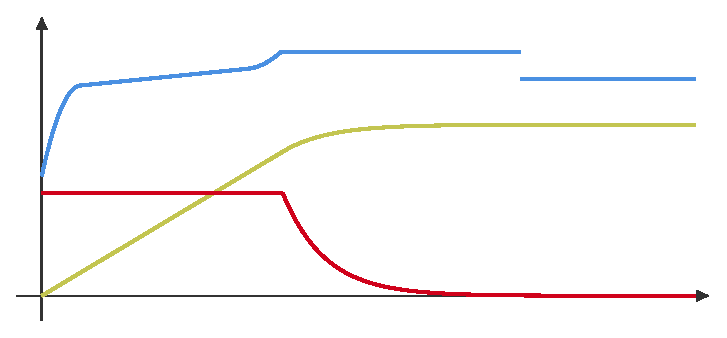
\includegraphics[width=332.25pt,height=145.5pt]{images/image_cccv}};
%Straight Lines [id:da8771255477316724] 
\draw [color={rgb, 255:red, 155; green, 155; blue, 155 }  ,draw opacity=1 ] [dash pattern={on 4.5pt off 4.5pt}]  (422,228.5) -- (422,360) ;
%Shape: Circle [id:dp0014709299474531257] 
\draw  [fill={rgb, 255:red, 255; green, 255; blue, 255 }  ,fill opacity=1 ] (268,203) .. controls (268,201.9) and (268.9,201) .. (270,201) .. controls (271.1,201) and (272,201.9) .. (272,203) .. controls (272,204.1) and (271.1,205) .. (270,205) .. controls (268.9,205) and (268,204.1) .. (268,203) -- cycle ;
%Shape: Circle [id:dp8257690320080588] 
\draw  [fill={rgb, 255:red, 255; green, 255; blue, 255 }  ,fill opacity=1 ] (268,267) .. controls (268,265.9) and (268.9,265) .. (270,265) .. controls (271.1,265) and (272,265.9) .. (272,267) .. controls (272,268.1) and (271.1,269) .. (270,269) .. controls (268.9,269) and (268,268.1) .. (268,267) -- cycle ;
%Straight Lines [id:da48605435215358694] 
\draw [color={rgb, 255:red, 74; green, 144; blue, 226 }  ,draw opacity=1 ][line width=1.5]  [dash pattern={on 1.69pt off 2.76pt}]  (422,207.7) -- (422,217.2) ;
%Straight Lines [id:da6398477641060736] 
\draw    (272,399) -- (420,399) ;
\draw [shift={(422,399)}, rotate = 180] [color={rgb, 255:red, 0; green, 0; blue, 0 }  ][line width=0.75]    (10.93,-3.29) .. controls (6.95,-1.4) and (3.31,-0.3) .. (0,0) .. controls (3.31,0.3) and (6.95,1.4) .. (10.93,3.29)   ;
\draw [shift={(270,399)}, rotate = 0] [color={rgb, 255:red, 0; green, 0; blue, 0 }  ][line width=0.75]    (10.93,-3.29) .. controls (6.95,-1.4) and (3.31,-0.3) .. (0,0) .. controls (3.31,0.3) and (6.95,1.4) .. (10.93,3.29)   ;
%Straight Lines [id:da7717485329022031] 
\draw    (118.5,399) -- (268,399) ;
\draw [shift={(270,399)}, rotate = 180] [color={rgb, 255:red, 0; green, 0; blue, 0 }  ][line width=0.75]    (10.93,-3.29) .. controls (6.95,-1.4) and (3.31,-0.3) .. (0,0) .. controls (3.31,0.3) and (6.95,1.4) .. (10.93,3.29)   ;
\draw [shift={(116.5,399)}, rotate = 0] [color={rgb, 255:red, 0; green, 0; blue, 0 }  ][line width=0.75]    (10.93,-3.29) .. controls (6.95,-1.4) and (3.31,-0.3) .. (0,0) .. controls (3.31,0.3) and (6.95,1.4) .. (10.93,3.29)   ;
%Straight Lines [id:da8998950689600032] 
\draw    (116,394) -- (116,404) ;
%Straight Lines [id:da17048346486898192] 
\draw    (270,394) -- (270,404) ;
%Straight Lines [id:da8039553388960854] 
\draw    (422,394) -- (422,404) ;
%Straight Lines [id:da2911914982770165] 
\draw [color={rgb, 255:red, 74; green, 144; blue, 226 }  ,draw opacity=1 ]   (78,124) -- (103,124) ;
%Straight Lines [id:da500593174587459] 
\draw [color={rgb, 255:red, 208; green, 2; blue, 27 }  ,draw opacity=1 ]   (78,144) -- (103,144) ;
%Straight Lines [id:da47080918502581004] 
\draw [color={rgb, 255:red, 195; green, 197; blue, 81 }  ,draw opacity=1 ]   (78,164) -- (103,164) ;

%Straight Lines [id:da7924785218065409] 
\draw [color={rgb, 255:red, 155; green, 155; blue, 155 }  ,draw opacity=1 ] [dash pattern={on 4.5pt off 4.5pt}]  (117,249) -- (533,249) ;

% Text Node
\draw (106,117.4) node [anchor=north west][inner sep=0.75pt]  [font=\footnotesize]  {$U_{\mathrm{B}}( t)$};
% Text Node
\draw (106,137.4) node [anchor=north west][inner sep=0.75pt]  [font=\footnotesize]  {$I_{\mathrm{B}}( t)$};
% Text Node
\draw (106,157.4) node [anchor=north west][inner sep=0.75pt]  [font=\footnotesize]  {$Q_{\mathrm{B}}( t)$};
% Text Node
\draw (547,352.4) node [anchor=north west][inner sep=0.75pt]  [font=\footnotesize]  {$t$};
% Text Node
\draw (142,382) node [anchor=north west][inner sep=0.75pt]  [font=\footnotesize] [align=left] {Constant current};
% Text Node
\draw (294,382) node [anchor=north west][inner sep=0.75pt]  [font=\footnotesize] [align=left] {Constant voltage};
% Text Node
\draw (102,363.4) node [anchor=north west][inner sep=0.75pt]  [font=\footnotesize]  {$0$};
% Text Node
\draw (84.5,242.4) node [anchor=north west][inner sep=0.75pt]  [font=\footnotesize]  {$Q_{\mathrm{tot}}$};
% Text Node
\draw (87,198.4) node [anchor=north west][inner sep=0.75pt]  [font=\scriptsize]  {$U_{\mathrm{full}}$};
% Text Node
\draw (97.2,287.4) node [anchor=north west][inner sep=0.75pt]  [font=\scriptsize]  {$I_{\mathrm{C}}$};
% Text Node
\draw (263,362.4) node [anchor=north west][inner sep=0.75pt]  [font=\footnotesize]  {$t_{\mathrm{C}}$};
% Text Node
\draw (400,362.4) node [anchor=north west][inner sep=0.75pt]  [font=\footnotesize]  {$t_{\mathrm{C}} +t_{\mathrm{V}}$};
% Text Node
\draw (60.5,259.4) node [anchor=north west][inner sep=0.75pt]  [font=\footnotesize]  {$Q_{\mathrm{B}}( t_{\mathrm{CC}})$};


\end{tikzpicture}






	\caption{An example of the behavior the battery voltage $U_\mathrm{B}(t)$, battery current $I_\mathrm{B}(t)$ and battery charge $Q_\mathrm{B}(t)$ of a $\mathrm{LiFePO}_4$ battery when it is charged with a constant current $I_\mathrm{C}$ and then with a constant voltage $U_\mathrm{full}$ over a longer period of time. At $t_\mathrm{C} + t_\mathrm{V}$ the battery charger switches from $U_\mathrm{full}$ to $U_\mathrm{float}$ to keep the battery in a fully charged state. (Recreated from: \cite{Notten:2005, Sterner:2017, Liu:2020})}
	\label{fig:tikz_cccv_curve}
\end{figure} 

With the \emph{charge difference} $\Delta Q = Q_\mathrm{tot} - Q_\mathrm{B}(t_\mathrm{C})$ and the model proposed in \cite{Liu:2020}, the battery charge can be written as a function of the charging time as follows: 
\begin{equation} \label{eq:battery_charge_cases}
\centering
		Q_\mathrm{B}(t) =
  		\begin{cases}
   			I_\mathrm{C} \, t \text{,} & \text{for } 0\mathrm{h} \leq t < t_\mathrm{C} 
			\\
    		\Delta Q \left( 1 - \exp \left( -\dfrac{t - t_\mathrm{C}}{\tau_\mathrm{B}} \right) \right) + I_\mathrm{C} \, t_\mathrm{C}\text{,} & \text{for } t_\mathrm{C} \leq t < t_\mathrm{C} + t_\mathrm{V} \text{.}
  		\end{cases}
\end{equation}
It is assumed that $Q_\mathrm{B}(t)$ is continuously differentiable for all points in time. Based on this assumption, the model for the charging current results from the time derivative: 
\begin{equation} \label{current_cases}
\dfrac{\mathrm{d}Q_\mathrm{B}(t)}{\mathrm{d}t} = 
	\left\{\begin{array}{ll}
		I_\mathrm{C}\text{,} & \text{for } 0\mathrm{h} \leq t < t_\mathrm{C} \\[8pt]
		\dfrac{\Delta Q}{\tau_\mathrm{B}} \exp \left( -\dfrac{t - t_\mathrm{C}}{\tau_\mathrm{B}} \right)\text{,} & \text{for } t_\mathrm{C} \leq t < t_\mathrm{C} + t_\mathrm{V}
 	\end{array}\right\} = I_\mathrm{B}(t) \text{.}
\end{equation}
If it is further assumed that $I_\mathrm{B}(t)$ is continuous for all points in time -- therefore does not drop at the point in time $t_\mathrm{C}$ -- the \emph{time constant} $\tau_\mathrm{B}$ in $\left(\mathrm{h}\right)$ of a battery can be obtained from:
\begin{equation}\label{eq:tau_battery}
	\centering
	\tau_\mathrm{B} = \dfrac{\Delta Q}{I_\mathrm{C}}\text{.}
\end{equation}
If -- in the course of the charge experiment -- it can be shown that the second assumption is correct, then the first assumption follows according to \cite{Taschner:2014}.
	
Like the discharge experiment, this experiment is also carried out at $\vartheta_\mathrm{A} = 25^\circ \mathrm{C}$. The $\mathrm{LiFePO}_4$ battery, however, is initially fully discharged ($\mathrm{SOC}_{1} = 0$) and the charging experiment is repeated for the desired number of measuring points $N_{\mathrm{MP}}$ until it is fully charged ($\mathrm{SOC}_{N_\mathrm{MP}} = 1$) \cite{Rahmoun:2012, Hentunen:2014, Gurjer:2019}.

The corresponding measurement setup can be seen in the figure \ref{fig:tikz_experiment_2}. For the currents $I_\mathrm{Ch1}$ and $I_\mathrm{Ch2}$ the same applies as in the discharge experiment since they are small compared to the \emph{battery charger current} $I_\mathrm{BC}$ in $\left(\mathrm{A}\right)$ \cite{Schrufer:2014}.
\begin{figure}[h!]
	\centering
	

\tikzset{every picture/.style={line width=0.75pt}} %set default line width to 0.75pt        

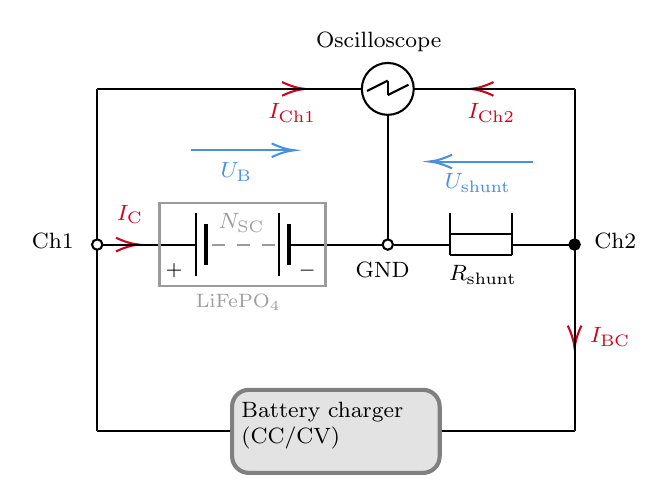
\begin{tikzpicture}[x=0.75pt,y=0.75pt,yscale=-1,xscale=1]
%uncomment if require: \path (0,748); %set diagram left start at 0, and has height of 748

%Straight Lines [id:da030470885996142894] 
\draw [color={rgb, 255:red, 208; green, 2; blue, 27 }  ,draw opacity=1 ]   (360,170) ;
\draw [shift={(360,170)}, rotate = 180] [color={rgb, 255:red, 208; green, 2; blue, 27 }  ,draw opacity=1 ][line width=0.75]    (10.93,-3.29) .. controls (6.95,-1.4) and (3.31,-0.3) .. (0,0) .. controls (3.31,0.3) and (6.95,1.4) .. (10.93,3.29)   ;
%Straight Lines [id:da3824823238969528] 
\draw [color={rgb, 255:red, 208; green, 2; blue, 27 }  ,draw opacity=1 ]   (570,205) -- (570,218) ;
\draw [shift={(570,220)}, rotate = 270] [color={rgb, 255:red, 208; green, 2; blue, 27 }  ,draw opacity=1 ][line width=0.75]    (10.93,-3.29) .. controls (6.95,-1.4) and (3.31,-0.3) .. (0,0) .. controls (3.31,0.3) and (6.95,1.4) .. (10.93,3.29)   ;
%Straight Lines [id:da5182691574210985] 
\draw    (340,260) -- (407.5,260) ;
%Straight Lines [id:da26468661252829784] 
\draw    (502.5,260) -- (570,260) ;
%Rounded Rect [id:dp15109738720083965] 
\draw  [color={rgb, 255:red, 128; green, 128; blue, 128 }  ,draw opacity=1 ][fill={rgb, 255:red, 227; green, 227; blue, 227 }  ,fill opacity=1 ][line width=1.5]  (405,248) .. controls (405,243.58) and (408.58,240) .. (413,240) -- (497,240) .. controls (501.42,240) and (505,243.58) .. (505,248) -- (505,272) .. controls (505,276.42) and (501.42,280) .. (497,280) -- (413,280) .. controls (408.58,280) and (405,276.42) .. (405,272) -- cycle ;
%Straight Lines [id:da04571217565366692] 
\draw [color={rgb, 255:red, 208; green, 2; blue, 27 }  ,draw opacity=1 ]   (535,95) -- (522,95) ;
\draw [shift={(520,95)}, rotate = 360] [color={rgb, 255:red, 208; green, 2; blue, 27 }  ,draw opacity=1 ][line width=0.75]    (10.93,-3.29) .. controls (6.95,-1.4) and (3.31,-0.3) .. (0,0) .. controls (3.31,0.3) and (6.95,1.4) .. (10.93,3.29)   ;
%Straight Lines [id:da286200132644544] 
\draw    (342,170) -- (370,170) ;
%Straight Lines [id:da17958881147308237] 
\draw    (450.5,170) -- (477.5,170) ;
%Straight Lines [id:da5043205087506204] 
\draw [color={rgb, 255:red, 208; green, 2; blue, 27 }  ,draw opacity=1 ]   (425,95) -- (438,95) ;
\draw [shift={(440,95)}, rotate = 180] [color={rgb, 255:red, 208; green, 2; blue, 27 }  ,draw opacity=1 ][line width=0.75]    (10.93,-3.29) .. controls (6.95,-1.4) and (3.31,-0.3) .. (0,0) .. controls (3.31,0.3) and (6.95,1.4) .. (10.93,3.29)   ;
%Straight Lines [id:da8819726416071505] 
\draw [line width=0.75]    (387.5,155) -- (387.5,185) ;
%Straight Lines [id:da22364644407030787] 
\draw [color={rgb, 255:red, 155; green, 155; blue, 155 }  ,draw opacity=1 ] [dash pattern={on 4.5pt off 4.5pt}]  (425.5,170) -- (390.5,170) ;
%Straight Lines [id:da8171048209291414] 
\draw [line width=1.5]    (392.5,160) -- (392.5,180) ;
%Straight Lines [id:da3784748951709651] 
\draw [line width=0.75]    (427.5,155) -- (427.5,185) ;
%Straight Lines [id:da23453075334713613] 
\draw [line width=1.5]    (432.5,160) -- (432.5,180) ;
%Straight Lines [id:da7174267672251604] 
\draw    (387.5,170) -- (370.5,170) ;
%Straight Lines [id:da8824908036219616] 
\draw    (449.5,170) -- (432.5,170) ;
%Shape: Rectangle [id:dp6355233140968859] 
\draw  [color={rgb, 255:red, 155; green, 155; blue, 155 }  ,draw opacity=1 ] (450,150) -- (450,190) -- (370,190) -- (370,150) -- cycle ;
%Shape: Circle [id:dp4046675137999993] 
\draw   (477.5,170) .. controls (477.5,168.62) and (478.62,167.5) .. (480,167.5) .. controls (481.38,167.5) and (482.5,168.62) .. (482.5,170) .. controls (482.5,171.38) and (481.38,172.5) .. (480,172.5) .. controls (478.62,172.5) and (477.5,171.38) .. (477.5,170) -- cycle ;
%Shape: Circle [id:dp8699232468402804] 
\draw   (337.5,170) .. controls (337.5,168.62) and (338.62,167.5) .. (340,167.5) .. controls (341.38,167.5) and (342.5,168.62) .. (342.5,170) .. controls (342.5,171.38) and (341.38,172.5) .. (340,172.5) .. controls (338.62,172.5) and (337.5,171.38) .. (337.5,170) -- cycle ;
%Straight Lines [id:da0932789662810869] 
\draw    (340,95) -- (340,167.5) ;
%Straight Lines [id:da7259313392072295] 
\draw    (340,95) -- (467.5,95) ;
%Straight Lines [id:da7181235672344906] 
\draw [color={rgb, 255:red, 74; green, 144; blue, 226 }  ,draw opacity=1 ]   (385,124.57) -- (433,124.57) ;
\draw [shift={(435,124.57)}, rotate = 180] [color={rgb, 255:red, 74; green, 144; blue, 226 }  ,draw opacity=1 ][line width=0.75]    (10.93,-3.29) .. controls (6.95,-1.4) and (3.31,-0.3) .. (0,0) .. controls (3.31,0.3) and (6.95,1.4) .. (10.93,3.29)   ;
%Shape: Circle [id:dp9954794574731103] 
\draw   (467.5,95) .. controls (467.5,88.1) and (473.1,82.5) .. (480,82.5) .. controls (486.9,82.5) and (492.5,88.1) .. (492.5,95) .. controls (492.5,101.9) and (486.9,107.5) .. (480,107.5) .. controls (473.1,107.5) and (467.5,101.9) .. (467.5,95) -- cycle ;
%Straight Lines [id:da04493405460274014] 
\draw    (470,96) -- (480,91) ;
%Straight Lines [id:da3033269159759058] 
\draw    (480,91) -- (480,98) ;
%Straight Lines [id:da8245646456208624] 
\draw    (480,98) -- (490,93) ;

%Straight Lines [id:da664654756239323] 
\draw    (340,172.5) -- (340,260) ;
%Straight Lines [id:da020631229787501093] 
\draw    (570,170) -- (570,260) ;
%Straight Lines [id:da42439143356479936] 
\draw    (492.5,95) -- (570,95) ;
%Straight Lines [id:da8878395010937925] 
\draw    (540,175) -- (540,165) ;
%Straight Lines [id:da5068559712609504] 
\draw    (510,175) -- (510,165) ;
%Straight Lines [id:da17027035780260014] 
\draw    (510,175) -- (540,175) ;
%Straight Lines [id:da7267594413628695] 
\draw    (510,165) -- (540,165) ;
%Straight Lines [id:da6452827698871475] 
\draw    (510,155) -- (510,165) ;
%Straight Lines [id:da9670069496965643] 
\draw    (540,155) -- (540,165) ;
%Shape: Circle [id:dp9967471299276287] 
\draw  [fill={rgb, 255:red, 0; green, 0; blue, 0 }  ,fill opacity=1 ] (570,167.5) .. controls (571.38,167.5) and (572.5,168.62) .. (572.5,170) .. controls (572.5,171.38) and (571.38,172.5) .. (570,172.5) .. controls (568.62,172.5) and (567.5,171.38) .. (567.5,170) .. controls (567.5,168.62) and (568.62,167.5) .. (570,167.5) -- cycle ;
%Straight Lines [id:da6778579527436412] 
\draw    (540,170) -- (570,170) ;
%Straight Lines [id:da9391362233033829] 
\draw    (483,170) -- (510,170) ;
%Straight Lines [id:da8151174249515367] 
\draw    (480,107.5) -- (480,167.5) ;
%Straight Lines [id:da4990891660653225] 
\draw [color={rgb, 255:red, 74; green, 144; blue, 226 }  ,draw opacity=1 ]   (550,130) -- (502,130) ;
\draw [shift={(500,130)}, rotate = 360] [color={rgb, 255:red, 74; green, 144; blue, 226 }  ,draw opacity=1 ][line width=0.75]    (10.93,-3.29) .. controls (6.95,-1.4) and (3.31,-0.3) .. (0,0) .. controls (3.31,0.3) and (6.95,1.4) .. (10.93,3.29)   ;
%Straight Lines [id:da37596819517946445] 
\draw    (570,95) -- (570,167.5) ;

% Text Node
\draw (576,208.4) node [anchor=north west][inner sep=0.75pt]  [font=\footnotesize,color={rgb, 255:red, 208; green, 2; blue, 27 }  ,opacity=1 ]  {$I_{\mathrm{BC}}$};
% Text Node
\draw (348,149.4) node [anchor=north west][inner sep=0.75pt]  [font=\footnotesize,color={rgb, 255:red, 208; green, 2; blue, 27 }  ,opacity=1 ]  {$I_{\mathrm{C}}$};
% Text Node
\draw (408,244.5) node [anchor=north west][inner sep=0.75pt]  [font=\footnotesize] [align=left] {Battery charger\\(CC/CV)};
% Text Node
\draw (386,192.4) node [anchor=north west][inner sep=0.75pt]  [font=\scriptsize,color={rgb, 255:red, 0; green, 0; blue, 0 }  ,opacity=1 ]  {$\mathrm{\textcolor[rgb]{0.61,0.61,0.61}{LiFePO}\textcolor[rgb]{0.61,0.61,0.61}{_{4}}}$};
% Text Node
\draw (435.5,177.4) node [anchor=north west][inner sep=0.75pt]  [font=\scriptsize]  {$-$};
% Text Node
\draw (371.5,177.4) node [anchor=north west][inner sep=0.75pt]  [font=\scriptsize]  {$+$};
% Text Node
\draw (397,153.4) node [anchor=north west][inner sep=0.75pt]  [font=\footnotesize,color={rgb, 255:red, 155; green, 155; blue, 155 }  ,opacity=1 ]  {$N_{\mathrm{SC}}$};
% Text Node
\draw (398,128.97) node [anchor=north west][inner sep=0.75pt]  [font=\footnotesize,color={rgb, 255:red, 74; green, 144; blue, 226 }  ,opacity=1 ]  {$U_{\mathrm{B}}$};
% Text Node
\draw (421,100.4) node [anchor=north west][inner sep=0.75pt]  [font=\footnotesize,color={rgb, 255:red, 208; green, 2; blue, 27 }  ,opacity=1 ]  {$I_{\mathrm{Ch} 1}$};
% Text Node
\draw (444,66) node [anchor=north west][inner sep=0.75pt]  [font=\footnotesize] [align=left] {Oscilloscope};
% Text Node
\draw (508,178.4) node [anchor=north west][inner sep=0.75pt]  [font=\footnotesize]  {$R_{\mathrm{shunt}}$};
% Text Node
\draw (506,134.4) node [anchor=north west][inner sep=0.75pt]  [font=\footnotesize,color={rgb, 255:red, 74; green, 144; blue, 226 }  ,opacity=1 ]  {$U_{\mathrm{shunt}}$};
% Text Node
\draw (517,100.4) node [anchor=north west][inner sep=0.75pt]  [font=\footnotesize,color={rgb, 255:red, 208; green, 2; blue, 27 }  ,opacity=1 ]  {$I_{\mathrm{Ch} 2}$};
% Text Node
\draw (463,177) node [anchor=north west][inner sep=0.75pt]  [font=\footnotesize] [align=left] {GND};
% Text Node
\draw (578,163) node [anchor=north west][inner sep=0.75pt]  [font=\footnotesize] [align=left] {Ch2};
% Text Node
\draw (307,163) node [anchor=north west][inner sep=0.75pt]  [font=\footnotesize] [align=left] {Ch1};


\end{tikzpicture}

	\caption{Measurement setup for the charge experiment.}
	\label{fig:tikz_experiment_2}
\end{figure}
Based on the figure \ref{fig:tikz_experiment_2}, the actual charging current $I_\mathrm{C}$ can be calculated with the equation (\ref{eq:i_c_real}).
\begin{equation}\label{eq:i_c_real}
	\centering
I_\mathrm{C} = -\dfrac{U_\mathrm{shunt}}{R_\mathrm{shunt}} - I_\mathrm{Ch1} - I_\mathrm{Ch2}
\end{equation}

Identical to the discharge experiment, the battery's open-circuit voltage $U_{0, \mathrm{C}}(\mathrm{SOC}_n)$ in $\left(\mathrm{V}\right)$ is measured with Ch1. The battery is then charged using a suitable battery charger in (CC/CV) mode with a set $I_{\mathrm C}$, $I_\mathrm{min}$, $U_\mathrm{full}$ and $U_\mathrm{float}$. This is done for the time interval $\Delta t_{\mathrm{C}}$ until the new measuring point $\mathrm{SOC}_{n+1}$ is reached. At the point in time when the battery charger is switched on, the voltage rise $\Delta U_{\mathrm C}(\mathrm{SOC}_n)$ is measured with Ch1 and the voltage drop $U_\mathrm{shunt}(\mathrm{SOC}_n)$ with Ch2. After the charge process for $\Delta t_{\mathrm{C}}$ has been completed, the battery must remain idle for $t_\mathrm{rest}$ until the open-circuit voltage has reached an end value (compare to figure \ref{fig:tikz_pc_pd_battery_curve}). When this value is reached, the measurements can be repeated for $\mathrm{SOC}_{n + 1}$ \cite{Rahmoun:2012, Hentunen:2014, Gurjer:2019}. Based on the previously introduced model $\Delta U_{\mathrm C}(\mathrm{SOC}_{N_\mathrm{MP}})$ cannot be obtained. However, by performing the experiment on a commercially available $\mathrm{LiFePO}_4$ battery, it was found that for longer resting periods $t_\mathrm{rest}$, of up to a few hours, it accepts small charging currents $I_{\mathrm C}$ for a short intervall $\Delta t_\mathrm{C}$ even for $\mathrm{SOC}_{N_\mathrm{MP}}$. It is assumed that this is the consequence of the slow -- almost exponential -- decrease of $U_{0, \mathrm{C}}(\mathrm{SOC}_{_\mathrm{MP}})$ (compare to figure \ref{fig:tikz_pc_pd_battery_curve}) \cite{Kurzweil:2018}. In this case, the equation (\ref{eq:battery_voltage}) is not equal to $U_{\mathrm{full}}$ anymore.

To confirm the previously made assumption that $I_{\mathrm C}(t)$ is continuous for all points in time, it is measured with Ch2 and calculated by using the equation (\ref{eq:i_c_real}) \cite{Notten:2005, Mertens:2015, Sterner:2017, Kurzweil:2018, Liu:2020}. 

The time interval $\Delta t_{\mathrm{C}}$ and the measuring points are calculated -- base on the Coulomb counting method -- as shown below \cite{He:2011, Wehbe:2015, Nejad:2016, Kurzweil:2018, Li:2018}:
\begin{equation} \label{eq:delta_t_C}
	\centering
	\Delta t_{\mathrm{C}} = \dfrac{ Q_\mathrm{tot}}{\eta_\mathrm{C} \, I_\mathrm{C} \left( N_\mathrm{MP} - 1 \right)} \text{.}
\end{equation}
\begin{equation} \label{eq:SOC_n_plus_1}
	\centering
	\mathrm{SOC}_{n + 1} = \mathrm{SOC}_{n} + \dfrac{\eta_\mathrm{C} \, I_\mathrm{C}}{Q_\mathrm{tot}} \, \Delta t_{\mathrm{C}} \text{.}
\end{equation}

Similar to $R_{e,\mathrm{D}}$, $R_{e,\mathrm{C}}$ can be obtained -- by using the equations (\ref{eq:r_0_c}) and (\ref{eq:i_c_real}) -- from \cite{Rahmoun:2012, Hentunen:2014, Kurzweil:2018, Gurjer:2019}:
\begin{equation}\label{eq:r_0_c_soc}
	\centering
	R_{\mathrm{e,C}}(\mathrm{SOC}_n) = \left|-\dfrac{\Delta U_{\mathrm C}(\mathrm{SOC}_n)}{\dfrac{U_\mathrm{shunt}(\mathrm{SOC}_n)}{R_\mathrm{shunt}} + I_\mathrm{Ch1} + I_\mathrm{Ch2}}\right| \text{.}
\end{equation}

Due to the hysteresis effects of the open-circuit voltage $U_0(\mathrm{SOC}_n)$ mentioned in \cite{Hentunen:2014, Wehbe:2015, Gurjer:2019, Saldana:2019}, the battery voltage in the equation (\ref{eq:battery_voltage}) must be adapted to the so-called \emph{zero-state hysteresis model}:

\begin{equation} \label{eq:battery_voltage_adapted}
	\centering
		U_\mathrm{B}(\mathrm{SOC}_n) =
  		\begin{cases}
   			U_0 (\mathrm{SOC}_n)+ \dfrac{c_{\mathrm{B}}}{2} - R_{\mathrm{e,D}}(\mathrm{SOC}_n) \, I_\mathrm{D}\text{,} \\ \text{when discharging the battery} \\[8pt]
    		U_0(\mathrm{SOC}_n) + \dfrac{c_{\mathrm{B}}}{2} + R_{\mathrm{e,C}}(\mathrm{SOC}_n) \, I_\mathrm{C}\text{,} \\\text{when charging the battery,}
  		\end{cases}
	\end{equation} 
with: 
\begin{equation} \label{eq:U_0}
	\centering
	U_0(\mathrm{SOC}_n) = \dfrac{U_{0,\mathrm{D}}(\mathrm{SOC}_n) + U_{0,\mathrm{C}}(\mathrm{SOC}_n)}{2}\text{,}
\end{equation}
and $c_{\mathrm{B}}$ depending on the sign of $I_\mathrm{B}$:
\begin{equation} \label{eq:c_B}
	\centering
		c_{\mathrm{B}} =
  		\begin{cases}
   			\left| U_{0, \mathrm{C}}(\mathrm{SOC}_n) - U_{0, \mathrm{D}}(\mathrm{SOC}_n) \right| \cdot (-1) \text{,} & \text{for } I_\mathrm{B} > 0\mathrm{A} \\
			0\text{,} & \text{for } I_\mathrm{B} = 0\mathrm{A} \\
			\left| U_{0, \mathrm{C}}(\mathrm{SOC}_n) - U_{0, \mathrm{D}}(\mathrm{SOC}_n) \right| \text{,} & \text{for } I_\mathrm{B} < 0\mathrm{A}\text{.}
  		\end{cases}
	\end{equation} 


